%% --------------------------------------------------------------------
%% Template UTEC Tesis
%% --------------------------------------------------------------------
% Este es el archivo que se debe compilar.
% 
% Este template ha sido modificado y actualizado por Eduardo Castro y Roosevelt Ubaldo en base a lo trabajado por Víctor Murray, Oscar Ramos y Juan Carlos Barbaran.
%
% Última actualización: Mayo, 2022

\documentclass[a4paper,12pt,oneside]{tesisutec}
\usepackage{longtable}
\selectlanguage{spanish}

%% Paquetes
\usepackage[utf8]{inputenc}
\usepackage[square, numbers, comma, sort&compress]{natbib}
% Libreria de idioma
\usepackage[spanish]{babel}
% Libreria para posicionamiento
\usepackage{float}
% Librerias para insertar codigos
\usepackage[spanish,onelanguage,ruled,vlined]{algorithm2e}
\usepackage{verbatim} 
% Librería para hipervínculos
\usepackage{hyperref}
 % Librería necesaria para arreglar el orden de referencias en overleaf.com
\usepackage{notoccite}

% Incluir acá los paquetes adicionales que deseas. 
% Ubicación de los imágenes.
\graphicspath{images/}

\makeatletter
% Reinsert missing \algbackskip
\def\algbackskip{\hskip-\ALG@thistlm}
\makeatother

\hypersetup{urlcolor=blue, colorlinks=true}

\begin{document}

\frontmatter

\department{CIENCIA DE LA COMPUTACIÓN}
\degree{Bachiller en Ciencia de la Computación}
\title{Mitigación de la resistencia evolutiva en glioblastoma multiforme mediante aprendizaje por refuerzo multiagente adversarial: optimización de políticas de terapia adaptativa bajo un marco MAPPO-CTDE con simulación calibrada}
\author{Kalos Brayan Lazo Mera \orcid{0000-0000-0000-0000} \\ Gianpier André Segovia Ureta \orcid{0000-0000-0000-0000}}
\supervisor{Victor Eduardo Martinez Abaunza \orcid{0000-0000-0000-0000}}
\date{2026}

\maketitle

\setstretch{1.5}


\input{encabezados/dedicatoria}
\input{encabezados/agradecimientos}

\tableofcontents

\newpage

\listoftables

\newpage

\listoffigures

\addtocontents{toc}{\vspace{1.5em}}

%% ============================================================================
\mainmatter
\pagestyle{fancy}

\input{secciones/resumen}
\input{secciones/abstract} 
\input{secciones/introduccion}
\chapter{INTRODUCCIÓN}
\label{cap:introduccion}

\section{Antecedentes}
\label{sec:antecedentes}

El glioblastoma multiforme (GBM) es el tumor cerebral primario maligno más frecuente y agresivo en adultos, con un pronóstico sombrío: a pesar del tratamiento multidisciplinario, la mediana de supervivencia global se mantiene en torno a los 12 a 15 meses y la supervivencia a cinco años no supera el 7\,\%~\cite{Tan2020,Sipos2025,Adegboyega2021}. El estándar de cuidado, conocido como protocolo de Stupp, consiste en la resección quirúrgica máxima segura seguida de radioterapia con temozolomida (TMZ) concurrente y adyuvante~\cite{Stupp2005,Jezierzanski2024}. Sin embargo, prácticamente todos los pacientes recaen: el tumor progresa o recurre con resistencia a la TMZ, y en el escenario de recurrencia no existe un estándar de cuidado establecido~\cite{Fernandes2017,Tan2020}.

Esta inevitabilidad de la recaída no es accidental, sino una consecuencia evolutiva del propio tratamiento. La administración a dosis máxima tolerada (MTD) ejerce una intensa presión selectiva que favorece la expansión de los subclones resistentes; al eliminar a las células sensibles se libera a las resistentes de la competencia por los recursos, acelerando su dominancia~\cite{Gatenby2022}. Frente a este fenómeno, la terapia adaptativa propone un cambio de paradigma: en lugar de buscar erradicar el tumor, busca \emph{contenerlo}, modulando la dosis para preservar deliberadamente una población sensible que compita con la resistente y retrase su expansión~\cite{Gallaher2017,Strobl2020}. Este enfoque, validado clínicamente en cáncer de próstata metastásico, prolongó significativamente el tiempo a progresión usando menos de la mitad de la dosis acumulada~\cite{Zhang2017}.

El reto, no obstante, es \emph{diseñar} el cronograma adaptativo óptimo. Dos líneas de investigación han abordado el problema desde ángulos complementarios. Por un lado, el aprendizaje por refuerzo (RL) ha demostrado poder descubrir políticas de dosificación que superan a los protocolos adaptativos heurísticos~\cite{Gallagher2024}. Por otro, la teoría de juegos ha formalizado el tratamiento como un juego de Stackelberg en el que el oncólogo es el líder y el tumor el seguidor evolutivo~\cite{Stankova2019}. Esta tesis se sitúa en la intersección de ambas líneas y formula una pregunta concreta: ¿cómo modelar la respuesta evolutiva del tumor como un \emph{adversario que aprende}, de modo que el aprendizaje por refuerzo descubra políticas de dosificación adaptativa que retrasen la resistencia en el glioblastoma?

\section{Planteamiento del problema}
\label{sec:problema}

El modelado computacional de la terapia adaptativa ha avanzado con rapidez, pero los enfoques actuales comparten una limitación en \emph{cómo representan la respuesta evolutiva del tumor}. Los métodos de RL para dosificación tratan al tumor como una dinámica fija sobre la que un único agente optimiza~\cite{Gallagher2024,Mashayekhi2023}: el tumor no anticipa ni responde estratégicamente. Las heurísticas de terapia adaptativa, aunque clínicamente exitosas, no se optimizan y aplican reglas fijas de encendido/apagado~\cite{Gallaher2017}. Los modelos teórico-de-juegos representan al tumor como un seguidor cuya respuesta se resuelve analíticamente o se asume racional~\cite{Stankova2019,Salvioli2024}, lo que limita la riqueza de comportamientos adversariales que el modelo puede capturar.

Esta omisión deja un conjunto recurrente de carencias. Las políticas resultantes no se entrenan contra el peor caso evolutivo, por lo que su robustez ante una respuesta tumoral estratégica queda sin verificar. Los modelos suelen ser genéricos o ilustrativos, sin calibración a datos reales de la enfermedad de interés. Y, de manera crítica, la evaluación tiende a recaer en métricas de carga tumoral aislada, que premian engañosamente la reducción agresiva del tumor ---precisamente la estrategia que induce la resistencia--- en lugar del desenlace clínico que importa: el tiempo durante el cual el tumor permanece manejable.

Trabajos recientes se aproximan al problema desde ángulos vecinos. El RL profundo aplicado a la programación adaptativa~\cite{Gallagher2024} demuestra el valor de las políticas aprendidas, pero sin adversario. Los marcos de juegos evolutivos de Stackelberg~\cite{Salvioli2024,Karima2025} capturan la asimetría líder-seguidor, pero resuelven al tumor analíticamente y rara vez se calibran. El RL adversarial robusto (RARL) muestra que entrenar contra un adversario que aprende mejora la estabilidad y la robustez de la política~\cite{Pinto2017}. Aun así, ninguno de estos enfoques modela simultáneamente a la terapia y al tumor como agentes de RL profundo que co-evolucionan adversarialmente sobre un simulador de GBM calibrado con datos reales, ni somete a prueba rigurosa si el entrenamiento con información centralizada (CTDE) aporta sobre el aprendizaje independiente. Esta es la brecha que la tesis aborda, y enmarcamos nuestra contribución como complemento de los paradigmas de RL de agente único y de juegos analíticos, no como su competidor.

\section{Pregunta de investigación e hipótesis}
\label{sec:pregunta}

A partir de la brecha anterior, la tesis se guía por una pregunta de investigación central:

\begin{quote}
\emph{¿En qué medida modelar el glioblastoma como un juego adversarial de dos agentes ---terapia y tumor--- resuelto mediante aprendizaje por refuerzo multiagente sobre un simulador calibrado con datos reales permite descubrir políticas de dosificación adaptativa que retrasen el tiempo hasta la dominancia resistente, en comparación con la dosis máxima tolerada y la heurística adaptativa de Gatenby; y aporta el crítico centralizado (CTDE) una ventaja sobre el aprendizaje independiente (IPPO) en este dominio?}
\end{quote}

Planteamos la hipótesis de que una política de terapia entrenada en \emph{self-play} adversarial contra un tumor que también aprende extiende el tiempo de manejo clínico exitoso ---definido como el número de días en que el tumor permanece simultáneamente controlado en carga y mayoritariamente tratable--- por encima tanto de la dosis máxima tolerada como de la heurística de Gatenby, de forma estadísticamente significativa sobre múltiples réplicas. Asimismo, planteamos que el mecanismo descubierto corresponde a una dosificación intermitente que preserva la competencia de las células sensibles, y caracterizamos empíricamente si el crítico centralizado mejora la fiabilidad del entrenamiento frente al aprendizaje independiente.

La hipótesis solo es contrastable si la evaluación no es engañosa: la métrica de éxito debe reflejar el desenlace clínico real y no la mera reducción de la carga. Por ello adoptamos una métrica de progresión auditada ---el tiempo a falla combinado, que termina el episodio cuando el tumor deja de estar controlado \emph{o} deja de ser tratable, reportando el motivo de falla--- en lugar de una métrica de carga aislada. Esta separación se incorpora por diseño y se detalla en el Capítulo~\ref{cap:metodologia}.

\section{Objetivos}
\label{sec:objetivos}

\subsection{Objetivo general}
\label{subsec:objetivo-general}

Diseñar un marco de aprendizaje por refuerzo multiagente adversarial ---GBMARL--- que modele la terapia y la resistencia evolutiva del glioblastoma como agentes en competencia sobre un simulador calibrado con datos reales, y evaluarlo cuantificando su capacidad para descubrir políticas de dosificación adaptativa que retrasen la intratabilidad frente a líneas base clínicas establecidas.

\subsection{Objetivos específicos}
\label{subsec:objetivos-especificos}

El objetivo general se descompone en cuatro objetivos específicos que organizan el trabajo metodológico de la tesis:

\begin{enumerate}
  \item Construir y calibrar un simulador de la dinámica tumoral sensible--resistente, basado en ecuaciones diferenciales ordinarias de competencia tipo Lotka-Volterra acopladas a la farmacodinámica de la temozolomida~\cite{Strobl2020,Yin2019}. La potencia del fármaco (concentración inhibitoria media y la brecha de sensibilidad entre poblaciones) se deriva de datos reales de sensibilidad de líneas celulares de GBM (GDSC2~\cite{GDSC} y DepMap~\cite{DepMap}), mientras que el techo de muerte celular se ancla a la literatura. Este objetivo actúa como compuerta de validación: el simulador debe reproducir el fracaso evolutivo de la dosis máxima tolerada por selección de resistencia.

  \item Formular el entorno de decisión multiagente con observabilidad parcial clínicamente justificada ---donde el agente de terapia no observa directamente la fracción resistente, replicando la limitación del oncólogo--- y una función de recompensa que optimice el desenlace clínico real (días con tumor controlado y tratable); e implementar el algoritmo MAPPO con entrenamiento centralizado y ejecución descentralizada (CTDE), junto con su variante de críticos independientes (IPPO)~\cite{Amato2024,deWitt2020}.

  \item Entrenar y validar las políticas aprendidas con múltiples semillas, reportando la significancia estadística de la mejora frente a las líneas base (dosis máxima tolerada y heurística de Gatenby) mediante una métrica de progresión auditada por modo de falla; e interpretar el mecanismo de la política resultante a partir de la trayectoria de dosificación.

  \item Aislar la contribución del crítico centralizado mediante una ablación controlada de CTDE frente a IPPO, y evaluar la sensibilidad del resultado a las constantes de calibración, para establecer en qué condiciones y por qué importa cada componente del marco.
\end{enumerate}

\section{Motivación}
\label{sec:motivacion}

Lo que justifica este trabajo no es solo la brecha identificada, sino la dificultad de cerrarla. El entrenamiento adversarial por \emph{self-play} es intrínsecamente inestable: la co-evolución de dos agentes puede asentarse en distintos equilibrios según la inicialización, produciendo resultados bimodales que exigen un protocolo de reproducibilidad y de reporte por tasa de éxito en lugar de promedios engañosos. Calibrar un simulador a partir de datos de sensibilidad \emph{in vitro} con el fin de optimizar un objetivo de \emph{control} dinámico es igualmente delicado, pues los datos informan la potencia del fármaco pero no la dinámica de competencia. Hacer que el entrenamiento sea estable, reproducible y honestamente evaluado constituye el núcleo técnico de la tesis.

La evaluación tiene un peso equivalente. La métrica de tiempo a falla combinado es clínicamente honesta por construcción: evita la trampa de premiar la reducción agresiva del tumor ---que minimiza la carga a corto plazo pero acelera la resistencia--- y mide en cambio el desenlace que de verdad importa. El beneficio esperado es práctico: una política adaptativa que retrase de forma robusta la dominancia resistente puede informar el diseño de cronogramas de temozolomida, y el marco es trasladable, en principio, a otros tumores gobernados por dinámicas evolutivas de resistencia.

\section{Alcance y limitaciones}
\label{sec:alcance}

Para mantener el argumento limpio y el trabajo dentro de un presupuesto de cómputo realista de pregrado, la tesis acota deliberadamente su alcance. El estudio es una validación \emph{in silico} sobre un simulador calibrado \emph{in vitro}, no una validación clínica. Nos centramos en el glioblastoma tratado con un único agente (temozolomida) y en un modelo no espacial de dos poblaciones (sensible y resistente); las extensiones a tratamientos combinados, a modelos espaciales y a otras histologías quedan como trabajo futuro. La calibración se realiza sobre el subconjunto de líneas celulares de GBM con genómica y ensayos completos disponibles, y la resistencia se modela como una transición fenotípica controlable ---respaldada por la evidencia de plasticidad fenotípica reversible~\cite{Boumahdi2019}--- en lugar de una mutación irreversible explícita. El entrenamiento se ejecuta en CPU con un hilo único para garantizar la reproducibilidad determinista, a costa de la velocidad.

Una limitación de fondo es que, con la calibración realista del glioblastoma, la resistencia resulta inevitable bajo cualquier estrategia que trate el tumor; esto refleja la realidad clínica de la enfermedad y delimita el objetivo de la tesis: \emph{retrasar} la intratabilidad, no curar ni eliminar el tumor. Reportamos además dos limitaciones de forma honesta: el entrenamiento adversarial exhibe bimodalidad, por lo que la tasa de éxito de contención prolongada no alcanza el 100\,\% de las réplicas; y el agente tumoral dispone de una palanca de acción limitada, lo que acota su capacidad de constituir una amenaza adversarial fuerte. En consecuencia, no afirmamos que el crítico centralizado sea universalmente superior, sino que caracterizamos honestamente cuándo aporta. Estas exclusiones no son concesiones, sino fronteras principistas que marcan el régimen en el que la contribución se sostiene sobre bases tanto evolutivas como estadísticas.

\section{Contribuciones}
\label{sec:contribuciones}

Esta tesis realiza las siguientes cuatro contribuciones, organizadas de la arquitectura a la evaluación:

\begin{enumerate}
  \item \textbf{Marco MARL adversarial calibrado (GBMARL).} Introducimos un marco que modela el tratamiento del glioblastoma como un juego adversarial de dos agentes ---terapia y tumor--- resuelto por aprendizaje por refuerzo multiagente. A diferencia de los enfoques de RL de agente único, que tratan al tumor como dinámica fija~\cite{Gallagher2024}, y de los marcos de juegos que resuelven al tumor analíticamente~\cite{Stankova2019,Salvioli2024}, en GBMARL ambos agentes son redes de RL profundo que co-evolucionan en \emph{self-play}, sobre un simulador específico de GBM calibrado con datos reales de sensibilidad farmacológica.

  \item \textbf{Política adaptativa descubierta y su mecanismo.} Mostramos que el marco descubre una política de dosificación que extiende el tiempo a la dominancia resistente por encima tanto de la dosis máxima tolerada como de la heurística adaptativa de Gatenby, de forma estadísticamente significativa. Además, interpretamos el mecanismo aprendido: una dosificación intermitente y modulada que preserva una población sensible competidora, redescubriendo de manera autónoma el principio de la terapia adaptativa.

  \item \textbf{Métrica de evaluación clínicamente honesta.} Formalizamos una métrica de tiempo a falla combinado, que mide los días en que el tumor permanece controlado en carga \emph{y} mayoritariamente tratable, reportando el modo de falla. Esta métrica evita los artefactos de las métricas de carga aislada ---que premian la reducción agresiva e inducen resistencia--- y se acompaña de un protocolo de validación multi-semilla con reporte por tasa de éxito y significancia estadística.

  \item \textbf{Estudio de ablación CTDE frente a IPPO en oncología.} Realizamos una ablación controlada que aísla el efecto del crítico centralizado, reportando de forma honesta en qué condiciones aporta sobre el aprendizaje independiente. Con ello retomamos, en el dominio nuevo de la terapia adaptativa, la pregunta abierta por de Witt et al.~\cite{deWitt2020} sobre la suficiencia del aprendizaje independiente.
\end{enumerate}

El resto de esta tesis se organiza como sigue. El Capítulo~\ref{cap:related-work} revisa críticamente la literatura en terapia adaptativa, modelos de resistencia, RL oncológico y modelos adversariales del cáncer. El Capítulo~\ref{cap:metodologia} presenta la arquitectura de GBMARL: el simulador calibrado, el entorno multiagente y la formulación adversarial MAPPO-CTDE. El Capítulo~\ref{cap:resultados} reporta la calibración, la validación multi-semilla, la comparación frente a las líneas base y la ablación CTDE. Finalmente, el Capítulo~\ref{cap:conclusiones} discute las limitaciones, los modos de falla y el trabajo futuro, y presenta las conclusiones.
\chapter{REVISIÓN CRÍTICA DE LA LITERATURA}
\label{cap:related-work}

Este capítulo sitúa a \textbf{GBMARL} ---el marco de aprendizaje por refuerzo multiagente (MARL) adversarial para terapia adaptativa en glioblastoma multiforme (GBM) que se propone en esta tesis--- dentro de seis vertientes convergentes de la literatura. Examinamos: (i)~la terapia adaptativa y la dinámica evolutiva de la resistencia como paradigma clínico; (ii)~los modelos matemáticos de competencia entre poblaciones sensibles y resistentes que fundamentan nuestro simulador; (iii)~el aprendizaje por refuerzo (RL) aplicado a la dosificación oncológica; (iv)~los modelos teórico-de-juegos y adversariales del cáncer, vecinos directos de nuestra formulación; (v)~los fundamentos de RL adversarial y multiagente (RARL, MAPPO, CTDE) sobre los que se construye el método; y (vi)~el modelado específico de la resistencia a la temozolomida (TMZ) en GBM. Mantenemos el alcance acotado: incluimos trabajos que (a)~modelan la resistencia evolutiva del tumor, (b)~optimizan la dosificación mediante control o aprendizaje, o (c)~aportan las primitivas algorítmicas de las que depende nuestro método.

Una tensión recorre las seis vertientes: \emph{cómo se representa la respuesta evolutiva del tumor}. Los enfoques existentes la modelan o bien no la modelan en absoluto (RL de dosificación sobre dinámicas tumorales fijas), o de forma heurística (terapia adaptativa de Gatenby), o como un \emph{seguidor racional resuelto analíticamente} (juegos de Stackelberg y control óptimo). Esa es precisamente la apertura que esta tesis ataca: ningún trabajo modela a ambos agentes ---terapia y tumor--- como aprendices de RL profundo que co-evolucionan adversarialmente sobre un simulador de GBM calibrado con datos reales. El capítulo se organiza alrededor de esa tensión y cierra con una síntesis metodológica y una declaración explícita de las brechas que motivan nuestras contribuciones.

\section{Terapia adaptativa y dinámica evolutiva de la resistencia}
\label{sec:terapia-adaptativa}

El estándar de cuidado en cánceres diseminados aplica la dosis máxima tolerada (MTD) buscando matar la mayor cantidad de células posible; sin embargo, esta estrategia ejerce una fuerte presión selectiva que favorece la expansión de subclones resistentes, y la recaída resulta casi inevitable~\cite{Gatenby2022}. La terapia adaptativa propone un cambio de objetivo: en lugar de erradicar, busca \emph{contener} el tumor explotando la competencia ecológica entre células sensibles y resistentes, preservando deliberadamente una población sensible que suprime el crecimiento de las resistentes~\cite{Gatenby2022,Zhang2023Review}.

La evidencia preclínica y de simulación es consistente. Gallaher et al.\ mostraron, con un modelo basado en agentes, que la modulación de dosis y los periodos de descanso controlan tumores heterogéneos suprimiendo espacialmente a las poblaciones resistentes menos aptas, mientras que la terapia continua a MTD conduce a recurrencia inevitable en presencia de cualquier célula resistente~\cite{Gallaher2017}. Hockings et al.\ confirmaron \emph{in vivo} en cáncer de ovario que adaptar la dosis a la respuesta tumoral prolonga significativamente la supervivencia sin aumentar la dosis media ni la toxicidad, aprovechando la menor aptitud de las células resistentes en ausencia de fármaco~\cite{Hockings2025}.

La validación clínica más influyente proviene del cáncer de próstata metastásico resistente a castración (mCRPC). Zhang et al.\ formularon un modelo de teoría de juegos evolutiva con ecuaciones de Lotka-Volterra y tres ``especies'' competidoras, y lo usaron para guiar ciclos de tratamiento de abiraterona según la dinámica tumoral de cada paciente; el ensayo piloto extendió el tiempo a progresión muy por encima del estándar usando menos de la mitad de la dosis acumulada~\cite{Zhang2017}. El seguimiento extendido reportó mejoras sostenidas en supervivencia libre de progresión y supervivencia global frente a una cohorte contemporánea con dosificación estándar~\cite{Zhang2022}. Este resultado es central para nuestra tesis: confirma que el valor de una estrategia evolutivamente informada no está en reducir el tumor, sino en \emph{retrasar} la dominancia resistente.

\section{Modelos matemáticos de la competencia sensible--resistente}
\label{sec:modelos-matematicos}

El simulador de GBMARL se apoya en la tradición de modelos de ecuaciones diferenciales ordinarias (EDO) para la dinámica tumoral y la evolución de la resistencia, revisados exhaustivamente por Yin et al.~\cite{Yin2019}. El núcleo de nuestro modelo ---dos poblaciones (sensible y resistente) en competencia logística tipo Lotka-Volterra--- sigue directamente a Strobl et al., quienes demostraron que el \emph{costo de resistencia} y la \emph{tasa de recambio} (turnover) celular determinan cuándo la terapia adaptativa logra extender el tiempo a progresión frente a la terapia continua~\cite{Strobl2020}. Estos dos parámetros son precisamente los que calibramos en nuestro simulador.

Trabajos posteriores refinan esta base. Masud et al.\ analizaron una dosificación evolutiva dependiente del tiempo sobre un modelo Lotka-Volterra, mostrando que un balance adecuado de la competencia permite la coexistencia estable de poblaciones por debajo de una carga tolerable~\cite{Masud2024}. Bao et al.\ caracterizaron el comportamiento biestable de poblaciones heterogéneas bajo farmacocinética, y hallaron que la resistencia preexistente contribuye más que la generada durante el tratamiento~\cite{Bao2023}.

Un aspecto clave de nuestro modelo es que la transición fenotípica sensible$\rightarrow$resistente se trata como una acción controlable del adversario, en lugar de una mutación irreversible. Esta elección está respaldada por la creciente evidencia de mecanismos \emph{no genéticos} de resistencia: Boumahdi y Sauvageau revisaron cómo la plasticidad fenotípica reversible y el cambio de estado celular (\emph{phenotype switching}) permiten a las células tolerar el fármaco y reganar sensibilidad tras su retirada~\cite{Boumahdi2019}. França et al.\ caracterizaron longitudinalmente este proceso como un ``continuo de resistencia'' de transiciones de estado celular con aptitud creciente~\cite{Franca2024}. Estos hallazgos justifican modelar la resistencia como un estado dinámico y maleable ---el sustrato sobre el que un adversario puede actuar.

\section{Aprendizaje por refuerzo para la dosificación oncológica}
\label{sec:rl-dosificacion}

La aplicación de RL a la programación de quimioterapia tiene una trayectoria consolidada, revisada por Yang et al.~\cite{Yang2022}. Los primeros trabajos, como Padmanabhan et al., usaron Q-learning sobre estados discretizados para el control en lazo cerrado de la dosis~\cite{Padmanabhan2017}. Mashayekhi et al.\ avanzaron hacia RL profundo en el espacio continuo original de estados y acciones, evitando la discretización guiada por expertos y reduciendo la duración del tratamiento y la dosis total administrada~\cite{Mashayekhi2023}.

El vecino más directo en esta vertiente es Gallagher et al., quienes aplicaron RL profundo para guiar la programación de terapia adaptativa en un modelo calibrado a próstata, superando los protocolos adaptativos vigentes y \emph{más que duplicando} el tiempo a progresión; además, destilaron políticas interpretables basadas en un único umbral de carga tumoral~\cite{Gallagher2024}. Su trabajo demuestra el potencial de RL para descubrir estrategias adaptativas superiores, pero adolece de una limitación que esta tesis aborda: trata al tumor como una dinámica fija (un único agente que aprende), sin modelar la respuesta evolutiva del tumor como un adversario que también aprende.

\section{Teoría de juegos y modelos adversariales del cáncer}
\label{sec:teoria-juegos}

Esta vertiente es la más adyacente a GBMARL y justifica nuestro encuadre ``adversarial''. La referencia fundacional es Staňková et al., quienes formularon el tratamiento del cáncer como un juego de Stackelberg con dos asimetrías: solo el médico juega racionalmente (el tumor únicamente se adapta a condiciones actuales) y existe una dinámica líder-seguidor en la que el oncólogo juega primero~\cite{Stankova2019}. El estándar de cuidado, al repetir el mismo fármaco hasta la progresión, desaprovecha ambas asimetrías.

Sobre esta base, Salvioli et al.\ compararon en un juego evolutivo de Stackelberg la MTD frente a una terapia ``evolutivamente ilustrada'' que anticipa tanto la respuesta ecológica como la evolución de la resistencia, hallando que esta última logra los mejores resultados con la menor dosis y la menor resistencia inducida~\cite{Salvioli2024}. Orlando et al.\ ya habían planteado el cáncer como un juego de control óptimo donde el oncólogo anticipa las adaptaciones del tumor explotando compromisos evolutivos~\cite{Orlando2012}. Romano et al.\ extendieron el marco a control basado en juegos evolutivos de Stackelberg y a un esquema de tres agentes tumor-inmune con liderazgo modulado~\cite{Romano2024,Romano2025}.

\subsection{Vecinos más cercanos y diferenciación}
\label{subsec:vecinos}

Dos trabajos recientes son los más próximos a esta tesis y, por ser un probable punto de escrutinio, merecen una diferenciación explícita. Tavakoli et al.\ integraron RL con teoría de juegos de Stackelberg sobre poblaciones sensibles y resistentes, aprendiendo políticas de dosificación que reducen resistencia y toxicidad~\cite{Tavakoli2025}. Karima et al.\ propusieron ``Nash-RL'', un marco que modela la interacción oncólogo-tumor como un juego de Stackelberg con un líder entrenado por RL y un seguidor evolutivo, mencionando RL multiagente y retraso de la resistencia~\cite{Karima2025}. Trivedi et al.\ implementaron un modelo basado en agentes con optimización de Stackelberg, logrando reducir la intensidad acumulada de tratamiento manteniendo el control~\cite{Trivedi2025}.

Tres diferencias separan a GBMARL de estos trabajos. \emph{Primero}, en todos ellos el tumor es un seguidor resuelto analíticamente o un agente evolutivo no aprendiente, mientras que en GBMARL ambos agentes son redes de RL profundo que co-evolucionan en \emph{self-play} adversarial. \emph{Segundo}, estos modelos son genéricos o ilustrativos (próstata, mama, o abstractos), mientras que GBMARL opera sobre un simulador \emph{específico de GBM calibrado con datos reales} de sensibilidad farmacológica (GDSC2~\cite{GDSC} y DepMap~\cite{DepMap}). \emph{Tercero}, Nash-RL en particular permanece como prueba de concepto sin calibración ni ablación arquitectónica, mientras que esta tesis estudia empíricamente el rol del crítico centralizado (CTDE frente a aprendizaje independiente) con una métrica de progresión auditada. GBMARL es, en suma, la realización empírica, calibrada y rigurosamente ablacionada de una idea que estos trabajos solo bosquejaron.

\section{Fundamentos de RL adversarial y multiagente}
\label{sec:fundamentos-marl}

El componente adversarial de GBMARL hereda del RL robusto. Pinto et al.\ introdujeron el RL adversarial robusto (RARL), donde un agente se entrena en presencia de un adversario que aprende una política de desestabilización óptima, formulando el aprendizaje como un objetivo minimax de suma cero; este esquema mejora la estabilidad del entrenamiento y la robustez de la política resultante~\cite{Pinto2017}. Huang et al.\ refinaron esta idea modelando el RL robusto como un juego de Stackelberg general en lugar de simultáneo de suma cero, lo que reduce la conservadurismo excesivo y la inestabilidad del entrenamiento~\cite{Huang2022}, un puente directo entre nuestra vertiente metodológica y la de teoría de juegos del cáncer. Daskalakis et al.\ aportaron garantías de convergencia para métodos de gradiente de política \emph{independientes} en juegos competitivos de dos agentes~\cite{Daskalakis2021}, resultado relevante para la variante IPPO que evaluamos.

En cuanto a la arquitectura multiagente, Amato ofrece la referencia introductoria de los paradigmas de entrenamiento centralizado con ejecución descentralizada (CTDE) y sus alternativas~\cite{Amato2024}. El algoritmo que adoptamos, MAPPO, emplea un crítico centralizado que accede al estado conjunto durante el entrenamiento mientras los actores ejecutan con observación local~\cite{Wang2025MAPPO}. Como contraparte, evaluamos la variante de críticos independientes (IPPO)~\cite{deWitt2020}; nuestra ablación CTDE retoma directamente la pregunta abierta por de Witt et al.\ sobre si el aprendizaje independiente es suficiente.

\section{Glioblastoma y resistencia a la temozolomida}
\label{sec:gbm-tmz}

El glioblastoma es incurable y su recurrencia resistente a TMZ es casi universal, lo que lo convierte en un caso paradigmático para una estrategia de contención evolutiva. Pérez-Aliacar et al.\ desarrollaron un modelo de adquisición de resistencia a TMZ en GBM basado en variables internas del estado fenotípico, calibrado con experimentos de esferoides 3D~\cite{PerezAliacar2024}; su enfoque respalda directamente nuestra metodología de calibración del simulador.

Dos trabajos aportan evidencia que \emph{respalda nuestro hallazgo principal} ---que espaciar y modular la dosis retrasa la resistencia. Segura-Collar et al.\ mostraron, mediante modelos validados y ensayos \emph{in silico}, que aumentar el tiempo entre dosis de TMZ reduce la toxicidad, retrasa la aparición de resistencias y mejora la supervivencia en GBM de crecimiento lento, mediado por cambios en el fenotipo tumoral~\cite{SeguraCollar2022}. Delobel et al.\ obtuvieron ganancias de supervivencia superiores a quince meses al introducir periodos de descanso entre dosis en gliomas, atribuidas al papel de las células persistentes en la resistencia~\cite{Delobel2023}. Sorribes et al.\ exploraron, desde el ángulo mecanístico, la combinación de TMZ con inhibición de la reparación del ADN~\cite{Sorribes2019}. En conjunto, esta línea confirma que la programación temporal de TMZ ---no solo su intensidad--- determina la dinámica de la resistencia, justo el grado de libertad que GBMARL optimiza.

\section{Temas transversales}
\label{sec:transversales}

Tres ejes metodológicos atraviesan la literatura revisada. \emph{Primero}, la representación del adversario evolutivo va desde su ausencia~\cite{Padmanabhan2017,Mashayekhi2023,Gallagher2024}, pasando por heurísticas de competencia~\cite{Gallaher2017,Strobl2020}, hasta seguidores racionales resueltos analíticamente~\cite{Stankova2019,Salvioli2024,Orlando2012}; GBMARL se sitúa en el extremo de un adversario co-aprendiente de RL profundo. \emph{Segundo}, la integración de aprendizaje va de nula, a RL de agente único~\cite{Gallagher2024,Mashayekhi2023}, a RL multiagente adversarial; nuestro trabajo se ubica en este último, combinando RARL~\cite{Pinto2017} con CTDE~\cite{Amato2024}. \emph{Tercero}, la calibración y evaluación oscila entre modelos genéricos ilustrativos y modelos calibrados a datos reales; GBMARL calibra con GDSC2/DepMap y evalúa con una métrica combinada de progresión y tratabilidad, en lugar de la métrica de carga aislada habitual.

\section{Brechas identificadas y justificación}
\label{sec:brechas}

Las seis vertientes dejan una brecha compuesta y específica que motiva esta tesis.

\subsection{Brecha en el modelado del adversario}
Ningún trabajo modela la respuesta evolutiva del tumor como un agente de RL profundo que \emph{aprende} en self-play adversarial. La línea de teoría de juegos~\cite{Stankova2019,Salvioli2024,Romano2024} resuelve al seguidor de forma analítica o asume juego racional; la línea de RL de dosificación~\cite{Gallagher2024,Mashayekhi2023} trata al tumor como dinámica fija. GBMARL cierra esta brecha entrenando terapia y tumor simultáneamente como adversarios, heredando la estabilidad y robustez documentadas para RARL~\cite{Pinto2017}.

\subsection{Brecha de calibración específica de GBM}
Los trabajos de RL y juegos se han centrado en próstata o mama~\cite{Zhang2017,Tavakoli2025}, o en modelos abstractos~\cite{Karima2025}. GBMARL ancla su simulador en datos reales de sensibilidad farmacológica de líneas de GBM (GDSC2~\cite{GDSC}, DepMap~\cite{DepMap}), en línea con la calibración experimental de Pérez-Aliacar et al.~\cite{PerezAliacar2024}.

\subsection{Brecha de rigor en la ablación arquitectónica}
La pregunta de si el crítico centralizado (CTDE) aporta sobre el aprendizaje independiente (IPPO) rara vez se somete a prueba en aplicaciones oncológicas. Retomando la hipótesis de de Witt et al.~\cite{deWitt2020}, GBMARL realiza una ablación controlada CTDE frente a IPPO y reporta el resultado de forma honesta, con una métrica de progresión auditada que evita los artefactos de las métricas de carga aisladas.

En suma, GBMARL no es una mejora marginal sobre una única línea base. Reúne, en un solo marco aprendido, (a)~el modelado del tumor como adversario co-aprendiente, (b)~un simulador de GBM calibrado con datos reales, y (c)~una evaluación rigurosa de la arquitectura CTDE con una métrica clínicamente honesta. La literatura revisada aporta los ingredientes por separado, pero ninguno de los trabajos los combina. Cerrar esa brecha compuesta es lo que esta tesis se propone.

\section{Tabla resumen}
\label{sec:tabla-resumen}

La Tabla~\ref{tab:related-work} resume los trabajos principales revisados y su relación con GBMARL.

% Requiere \usepackage{longtable} en el preámbulo (main.tex).
{\footnotesize
\renewcommand{\arraystretch}{1.25}
\begin{longtable}{@{}p{0.4cm}p{2.7cm}p{0.7cm}p{3.3cm}p{3.9cm}@{}}
\caption{Resumen de los trabajos principales revisados y su relación con GBMARL.}
\label{tab:related-work}\\
\hline
\textbf{\#} & \textbf{Trabajo} & \textbf{Año} & \textbf{Hallazgo clave} & \textbf{Relación con GBMARL} \\
\hline
\endfirsthead
\multicolumn{5}{l}{\textit{\tablename~\thetable{} -- continúa de la página anterior}}\\
\hline
\textbf{\#} & \textbf{Trabajo} & \textbf{Año} & \textbf{Hallazgo clave} & \textbf{Relación con GBMARL} \\
\hline
\endhead
\hline
\multicolumn{5}{r}{\textit{continúa en la página siguiente}}\\
\endfoot
\hline
\endlastfoot
1 & Zhang et al.~\cite{Zhang2017} & 2017 & Terapia adaptativa por juego evolutivo duplica el TTP en próstata & Validación clínica del paradigma de contención \\
2 & Strobl et al.~\cite{Strobl2020} & 2020 & Costo de resistencia y turnover rigen el éxito adaptativo & Base del modelo Lotka-Volterra que calibramos \\
3 & Gallaher et al.~\cite{Gallaher2017} & 2017 & Modulación de dosis suprime resistentes por competencia & Heurística que nuestro agente supera \\
4 & Gallagher et al.~\cite{Gallagher2024} & 2024 & RL profundo supera protocolos adaptativos en próstata & Vecino RL; tumor fijo, sin adversario \\
5 & Staňková et al.~\cite{Stankova2019} & 2019 & Tratamiento como juego de Stackelberg líder-seguidor & Encuadre adversarial fundacional \\
6 & Salvioli et al.~\cite{Salvioli2024} & 2024 & Terapia evolutivamente ilustrada vence a MTD en un SEG & Seguidor analítico; lo hacemos aprendiente \\
7 & Tavakoli et al.~\cite{Tavakoli2025} & 2025 & RL + Stackelberg en mama sensible/resistente & Vecino cercano; RL de agente único \\
8 & Karima et al.~\cite{Karima2025} & 2025 & Nash-RL: oncólogo-tumor como Stackelberg con RL & Vecino más cercano; sin calibración \\
9 & Pinto et al.~\cite{Pinto2017} & 2017 & RARL: adversario aprendiente mejora robustez & Fundamento del self-play adversarial \\
10 & Amato~\cite{Amato2024} & 2024 & Introducción a CTDE en MARL cooperativo & Paradigma de nuestro crítico centralizado \\
11 & de Witt et al.~\cite{deWitt2020} & 2020 & IPPO iguala o supera a métodos centralizados & Hipótesis que ablacionamos (CTDE vs.\ IPPO) \\
12 & Pérez-Aliacar et al.~\cite{PerezAliacar2024} & 2024 & Modelo de resistencia a TMZ en GBM calibrado a esferoides & Respalda nuestra calibración de GBM \\
13 & Segura-Collar et al.~\cite{SeguraCollar2022} & 2022 & Espaciar dosis de TMZ retrasa la resistencia en GBM & Respalda nuestro hallazgo principal \\
14 & Boumahdi y Sauvageau~\cite{Boumahdi2019} & 2019 & Plasticidad fenotípica reversible como resistencia & Justifica modelar la transición $\phi$ \\
15 & Yin et al.~\cite{Yin2019} & 2019 & Revisión de modelos EDO de dinámica y resistencia & Marco de modelado del simulador \\
\hline
\end{longtable}
}
\chapter{MARCO METODOLÓGICO}
\label{cap:metodologia}

Este capítulo describe GBMARL, el marco de aprendizaje por refuerzo multiagente adversarial propuesto para descubrir políticas de dosificación adaptativa en glioblastoma. La construcción sigue un principio de validación incremental, de adentro hacia afuera: primero se especifica y prueba el simulador de la dinámica tumoral (Sección~\ref{sec:simulador}); luego se calibra con datos reales de sensibilidad farmacológica (Sección~\ref{sec:calibracion}); a continuación se formula el problema de decisión como un juego adversarial de dos agentes (Sección~\ref{sec:juego}) con una función de recompensa alineada al desenlace clínico (Sección~\ref{sec:recompensa}); se entrena mediante el algoritmo MAPPO con entrenamiento centralizado y ejecución descentralizada (Sección~\ref{sec:algoritmo}); y, finalmente, se evalúa bajo un protocolo experimental con una métrica de progresión auditada (Sección~\ref{sec:protocolo}).

Este orden no es accidental: la ecuación diferencial es comprobable de forma aislada, y un agente único entrenado con PPO contra un tumor de comportamiento fijo permite verificar el entorno antes de introducir la complejidad del aprendizaje multiagente.

\section{Visión general del marco}
\label{sec:vision-general}

GBMARL modela el tratamiento del glioblastoma como un juego de suma no nula entre dos agentes que actúan sobre un mismo sistema dinámico:

\begin{itemize}
  \item El \textbf{agente de terapia} elige, en cada paso de decisión, la tasa de administración del fármaco $u(t)$; su objetivo es maximizar el tiempo durante el cual el tumor permanece clínicamente manejable.
  \item El \textbf{agente tumoral} controla la tasa de transición fenotípica $\phi$ de células sensibles a resistentes; su objetivo es forzar la dominancia de la población resistente.
\end{itemize}

Ambos agentes aprenden simultáneamente mediante \emph{self-play} sobre un simulador de ecuaciones diferenciales ordinarias (EDO). Es crucial subrayar que los datos experimentales \emph{solo calibran el simulador}: no se entrena ninguna red supervisada sobre datos de pacientes. Las políticas emergen de la interacción con el simulador calibrado, lo que sitúa el aprendizaje en un régimen de control óptimo bajo incertidumbre evolutiva, en lugar de un régimen de predicción supervisada.

\section{Simulador de la dinámica tumoral}
\label{sec:simulador}

El tumor se representa mediante dos poblaciones celulares en competencia: las sensibles $S$ y las resistentes $R$, junto con la concentración intratumoral del fármaco $c$. La dinámica sigue un modelo de competición logística tipo Lotka-Volterra acoplado a la farmacodinámica del fármaco~\cite{Strobl2020,Yin2019}:

\begin{align}
  \frac{dS}{dt} &= \alpha_S\, S\left(1 - \frac{S+R}{K}\right) - \delta_S(c)\,S - \phi\,S, \label{eq:ode-S}\\[4pt]
  \frac{dR}{dt} &= \alpha_R\, R\left(1 - \frac{S+R}{K}\right) - \delta_R(c)\,R + \phi\,S, \label{eq:ode-R}\\[4pt]
  \frac{dc}{dt} &= -\lambda_c\, c + u(t). \label{eq:ode-c}
\end{align}

Aquí $\alpha_S$ y $\alpha_R$ son las tasas de crecimiento intrínsecas, $K$ la capacidad de carga, y $\lambda_c$ la tasa de eliminación del fármaco. El término $\phi\,S$ representa la conversión fenotípica de sensibles a resistentes: aparece restado en~\eqref{eq:ode-S} y sumado en~\eqref{eq:ode-R}, lo que conserva la masa celular transferida. Modelar la resistencia como una transición fenotípica controlable ---y no como una mutación irreversible--- está respaldado por la evidencia de plasticidad fenotípica reversible en la resistencia no genética~\cite{Boumahdi2019}.

El efecto citotóxico del fármaco sobre cada población se modela con una función de Hill, que captura la respuesta sigmoide dosis-efecto característica de los ensayos de sensibilidad:

\begin{equation}
  \delta_X(c) = \delta_X^{\max}\, \frac{c^{\,h}}{\mathrm{IC50}_X^{\,h} + c^{\,h}}, \qquad X \in \{S, R\}, \label{eq:hill}
\end{equation}

donde $\delta_X^{\max}$ es la muerte celular máxima alcanzable, $\mathrm{IC50}_X$ la concentración que produce la mitad del efecto máximo, y $h$ el coeficiente de Hill. La diferencia clave entre poblaciones reside en que $\mathrm{IC50}_R \gg \mathrm{IC50}_S$: las células resistentes requieren concentraciones mucho mayores para ser afectadas.

El sistema~\eqref{eq:ode-S}--\eqref{eq:ode-c} se integra numéricamente mediante el método de Runge-Kutta de cuarto orden (RK4) con paso fijo $dt$. La implementación de la dinámica es matemática pura y se valida de forma aislada mediante pruebas unitarias: en ausencia de fármaco el tumor crece hasta la capacidad de carga; bajo dosis alta constante la población sensible decrece y la resistente se expande; y las poblaciones nunca toman valores negativos.

\section{Calibración del simulador con datos reales}
\label{sec:calibracion}

La calibración separa estrictamente lo que proviene de los datos de lo que proviene de la literatura. El principio rector es que \emph{los datos determinan la potencia del fármaco} (la posición de las curvas dosis-respuesta y la brecha de sensibilidad entre poblaciones), mientras que \emph{la literatura ancla el techo de muerte y las tasas de crecimiento}.

\subsection{Fuente y procesamiento de datos}

Las concentraciones inhibitorias se derivan de los ensayos de sensibilidad a temozolomida en líneas celulares de glioblastoma del repositorio GDSC2~\cite{GDSC}, cruzados con la anotación genómica de DepMap~\cite{DepMap}. El cruce entre ambos repositorios es un punto crítico: las claves de identificación deben normalizarse en ambos lados (mayúsculas y eliminación de caracteres no alfanuméricos) antes del mapeo, pues un cruce ingenuo por nombre pierde líneas en silencio. Tras la corrección, se recuperan 34 líneas de glioblastoma con ensayos de sensibilidad y 24 con genómica completa, frente a las 6 que recuperaba la versión defectuosa del cruce. Este saneamiento se documenta reportando explícitamente cuántas líneas se recuperan y por qué se descarta cada una.

De estos datos se estima la $\mathrm{IC50}$ de la población sensible y, a partir de la dispersión de respuestas, la $\mathrm{IC50}$ efectiva de la población resistente. El resultado es una brecha de sensibilidad de aproximadamente un orden de magnitud ($\mathrm{IC50}_R / \mathrm{IC50}_S \approx 9$), coherente con el carácter clínicamente refractario del glioblastoma a la temozolomida.

\subsection{Procedencia de los parámetros}

El techo de muerte $\delta_X^{\max}$ no se estima de datos \emph{in vitro} ---que no informan directamente la dinámica de competencia--- sino que se ancla a la literatura mediante una razón muerte-crecimiento, $\delta_S^{\max} = \kappa\, \alpha_S$ con $\kappa = 2{,}0$, garantizando que el fármaco disponga de palanca terapéutica suficiente. La Tabla~\ref{tab:procedencia} documenta la procedencia de cada parámetro, distinguiendo entre los derivados de \textbf{datos}, los anclados a \textbf{literatura}, y los fijados por \textbf{normalización} del modelo.

\begin{table}[H]
\centering
\caption{Procedencia de los parámetros del simulador. DATO: estimado de GDSC2/DepMap; LIT: anclado a literatura; NORM: fijado por normalización del modelo.}
\label{tab:procedencia}
\renewcommand{\arraystretch}{1.2}
\begin{tabular}{l|l|c|l}
\textbf{Parámetro} & \textbf{Símbolo} & \textbf{Valor} & \textbf{Procedencia} \\
\hline
Crecimiento sensibles      & $\alpha_S$        & 0.15  & LIT \\
Crecimiento resistentes    & $\alpha_R$        & 0.10  & LIT (costo de resistencia) \\
Capacidad de carga         & $K$               & 1.0   & NORM \\
Eliminación del fármaco    & $\lambda_c$       & 0.40  & LIT \\
Transición basal           & $\phi_{\text{base}}$ & 0.005 & LIT \\
IC50 sensibles             & $\mathrm{IC50}_S$ & 0.36  & DATO (GDSC2) \\
IC50 resistentes           & $\mathrm{IC50}_R$ & 3.27  & DATO (GDSC2) \\
Coeficiente de Hill        & $h$               & 2.0   & LIT \\
Muerte máx.\ sensibles     & $\delta_S^{\max}$ & 0.30  & LIT (anclada, $\kappa\,\alpha_S$) \\
Muerte máx.\ resistentes   & $\delta_R^{\max}$ & 0.15  & LIT (anclada) \\
\end{tabular}
\end{table}

Toda fórmula que transforma un dato en un parámetro de la EDO queda documentada de forma explícita, sin constantes mágicas sin derivación. Un hallazgo honesto de la calibración es que la temozolomida resulta un fármaco débil \emph{in vitro}, lo cual refleja fielmente la realidad clínica del glioblastoma como enfermedad incurable.

\section{Formulación como juego adversarial multiagente}
\label{sec:juego}

El problema de decisión se formula como un entorno multiagente paralelo siguiendo la interfaz \texttt{ParallelEnv} de PettingZoo~\cite{Terry2021}, con dos agentes que actúan de manera simultánea sobre el sistema~\eqref{eq:ode-S}--\eqref{eq:ode-c}. El estado dinámico real del sistema es tridimensional, $s = (S, R, c)$; los descriptores genómicos de la línea celular condicionan los parámetros iniciales a través de la calibración, pero no evolucionan durante el episodio.

\subsection{Observabilidad parcial}

Un elemento central del diseño es la observabilidad parcial clínicamente justificada. El agente de terapia no observa la composición interna del tumor, sino únicamente la carga total y la concentración del fármaco, replicando la limitación real del oncólogo, que no puede medir directamente la fracción resistente:

\begin{equation}
  o^{\text{ter}} = (S+R,\; c), \qquad o^{\text{tum}} = (S,\; R), \qquad s^{\text{global}} = (S, R, c). \label{eq:obs}
\end{equation}

Esta asimetría informativa es precisamente lo que motiva un crítico centralizado: durante el entrenamiento, el crítico puede acceder al estado conjunto $s^{\text{global}}$ ---incluida la fracción resistente que el actor de terapia no observa--- para realizar una mejor asignación de crédito.

\subsection{Espacios de acción}

La acción del agente de terapia es la tasa de dosificación $u \in [0, u_{\max}]$. La acción del agente tumoral es la tasa de transición fenotípica $\phi \in [0, \phi_{\max}]$. Acotar la acción del adversario es esencial: un adversario sin restricción puede forzar trivialmente la resistencia y degenerar en un \emph{hombre de paja} sin valor de modelado. La cota $\phi_{\max}$ y el costo de crecimiento implícito (la conversión drena la población sensible) imponen un compromiso evolutivo realista al tumor.

\section{Diseño de la función de recompensa}
\label{sec:recompensa}

El diseño de la recompensa fue iterativo y constituye, en sí mismo, un resultado metodológico. Documentamos su evolución de forma honesta porque ilustra una trampa conceptual recurrente.

\subsection{Evolución de la recompensa}

Una primera recompensa que penalizaba la carga tumoral instantánea ($r^{\text{ter}} = -(S+R)$) condujo al agente a redescubrir la estrategia de dosis máxima: minimizar la carga a corto plazo selecciona agresivamente la resistencia y pierde a largo plazo. Penalizar la fracción resistente con un peso fijo tampoco resolvió el problema: un peso alto hacía al agente abandonar el control de la carga, y un peso bajo lo hacía ignorar la resistencia. La lección es que \emph{minimizar el tamaño del tumor es el objetivo equivocado}; el objetivo correcto es maximizar el tiempo durante el cual el tumor permanece simultáneamente controlado y tratable.

\subsection{Recompensa final}

La formulación final premia directamente cada día de manejo clínico exitoso. Definimos dos condiciones sobre el estado:

\begin{align}
  \text{controlado} &: \quad S + R < \theta_{\text{prog}}, \label{eq:controlado}\\
  \text{tratable}   &: \quad \frac{R}{S+R} < \rho_{\text{may}}, \label{eq:tratable}
\end{align}

donde $\theta_{\text{prog}} = 0{,}8\,K$ es el umbral de progresión en carga y $\rho_{\text{may}} = 0{,}5$ el umbral de mayoría resistente. La recompensa del agente de terapia otorga una bonificación por cada día en que ambas condiciones se cumplen, menos un costo de toxicidad proporcional a la dosis:

\begin{equation}
  r^{\text{ter}} = b_{\text{ctrl}}\cdot \mathbb{1}[\text{controlado} \wedge \text{tratable}] - w_{\text{tox}}\, u, \label{eq:reward-ter}
\end{equation}

y el agente tumoral recibe una recompensa creciente con la fracción resistente más una bonificación al forzar la falla:

\begin{equation}
  r^{\text{tum}} = \frac{R}{S+R} + b_{\text{prog}}\cdot \mathbb{1}[\neg(\text{controlado} \wedge \text{tratable})]. \label{eq:reward-tum}
\end{equation}

El episodio termina cuando falla cualquiera de las dos condiciones, o por erradicación (con una bonificación $b_{\text{win}}$ para la terapia), o por truncamiento al alcanzar el horizonte. La Tabla~\ref{tab:hiperparametros-env} resume los valores adoptados.

\begin{table}[H]
\centering
\caption{Hiperparámetros del entorno y de la recompensa.}
\label{tab:hiperparametros-env}
\renewcommand{\arraystretch}{1.2}
\begin{tabular}{l|c||l|c}
\textbf{Parámetro} & \textbf{Valor} & \textbf{Parámetro} & \textbf{Valor} \\
\hline
Bonif.\ de control $b_{\text{ctrl}}$       & 1.0  & Umbral progresión $\theta_{\text{prog}}$ & $0.8\,K$ \\
Peso de toxicidad $w_{\text{tox}}$         & 0.05 & Umbral mayoría $\rho_{\text{may}}$        & 0.50 \\
Bonif.\ progresión $b_{\text{prog}}$       & 10.0 & Cota de transición $\phi_{\max}$          & 0.05 \\
Bonif.\ erradicación $b_{\text{win}}$      & 50.0 & Horizonte (días)                          & 180 \\
Estado inicial $S_0,\,R_0$                 & 0.40,\,0.01 & Paso de integración $dt$           & 0.1 \\
\end{tabular}
\end{table}

\section{Algoritmo de aprendizaje: MAPPO-CTDE}
\label{sec:algoritmo}

Las políticas se aprenden con una implementación propia en PyTorch de \emph{Multi-Agent Proximal Policy Optimization} (MAPPO)~\cite{Yu2022}, bajo el paradigma de entrenamiento centralizado y ejecución descentralizada (CTDE)~\cite{Amato2024}. Cada agente $i$ posee un actor $\pi_{\theta_i}(a^i \mid o^i)$ que actúa sobre su observación local, y comparte el marco de optimización de PPO~\cite{Schulman2017}.

\subsection{Crítico centralizado y estimación de ventajas}

El componente CTDE reside en el crítico. En la variante MAPPO, el crítico $V_{\psi_i}(s^{\text{global}})$ de cada agente accede al estado conjunto~\eqref{eq:obs} durante el entrenamiento, mientras que los actores ejecutan solo con su observación local. Las ventajas se estiman mediante \emph{Generalized Advantage Estimation} (GAE)~\cite{Schulman2016}:

\begin{equation}
  \hat{A}_t = \sum_{l=0}^{T-t-1} (\gamma\lambda)^l\, \delta_{t+l}, \qquad \delta_t = r_t + \gamma V_\psi(s_{t+1}) - V_\psi(s_t), \label{eq:gae}
\end{equation}

y cada actor se actualiza con el objetivo recortado de PPO:

\begin{equation}
  \mathcal{L}^{\text{PPO}}(\theta) = \mathbb{E}_t\!\left[\min\left(\varrho_t(\theta)\,\hat{A}_t,\; \mathrm{clip}(\varrho_t(\theta), 1-\epsilon, 1+\epsilon)\,\hat{A}_t\right)\right] + c_{\text{ent}}\, \mathcal{H}[\pi_\theta], \label{eq:ppo}
\end{equation}

donde $\varrho_t(\theta)$ es el cociente de probabilidades entre la política nueva y la antigua, y $\mathcal{H}$ el término de entropía que favorece la exploración. La naturaleza adversarial se introduce mediante \emph{self-play}: ambos agentes se entrenan simultáneamente, cada uno optimizando su propia recompensa contra la política actual del oponente, un esquema cuya estabilidad y robustez están respaldadas por el aprendizaje por refuerzo adversarial robusto~\cite{Pinto2017}.

\subsection{Variante de ablación: IPPO}

Para aislar empíricamente la contribución del crítico centralizado, se implementa la variante de aprendizaje independiente (IPPO)~\cite{deWitt2020}, idéntica en todo salvo en que el crítico $V_{\psi_i}(o^i)$ observa únicamente la observación local del agente, en lugar del estado conjunto. La comparación entre ambas variantes, manteniendo fijos el actor, la observación de ejecución y todos los hiperparámetros, aísla el efecto puro de CTDE.

\begin{algorithm}[H]
\SetAlgoLined
\KwIn{simulador calibrado, semilla, número de pasos $N$, modo (MAPPO/IPPO)}
\KwOut{políticas $\pi_{\theta_{\text{ter}}}$, $\pi_{\theta_{\text{tum}}}$}
Inicializar actores y críticos; fijar semillas y modo determinista\;
\While{pasos $< N$}{
  Recolectar trayectorias de \emph{self-play}: ambos agentes actúan sobre el simulador\;
  \For{cada agente $i \in \{\text{terapia}, \text{tumor}\}$}{
    Entrada del crítico $\gets s^{\text{global}}$ si MAPPO, o $o^i$ si IPPO\;
    Calcular ventajas $\hat{A}_t$ con GAE según~\eqref{eq:gae}\;
    Actualizar actor con el objetivo recortado~\eqref{eq:ppo} y crítico por regresión de valor\;
  }
}
\caption{Entrenamiento adversarial por self-play (MAPPO / IPPO).}
\label{alg:selfplay}
\end{algorithm}

\subsection{Reproducibilidad}

Dado que el entrenamiento adversarial por \emph{self-play} es intrínsecamente inestable y puede asentarse en distintos equilibrios según la inicialización, se impone un régimen determinista: ejecución en un solo hilo, activación de algoritmos deterministas y sembrado completo de los generadores aleatorios. Esto garantiza que una misma semilla produzca el mismo resultado dentro de un experimento, a costa de la velocidad de cómputo.

\section{Protocolo experimental y métricas de evaluación}
\label{sec:protocolo}

\subsection{Métrica de progresión auditada}

El desenlace se mide con el \textbf{tiempo a falla combinado} (TTP-combinado): el número de días hasta que el tumor deja de estar controlado~\eqref{eq:controlado} \emph{o} deja de ser tratable~\eqref{eq:tratable}, lo que ocurra primero, reportando además el \emph{motivo} de falla (progresión en carga, mayoría resistente o supervivencia al horizonte). Esta métrica es clínicamente honesta por construcción y evita un artefacto sutil: una métrica basada únicamente en la resistencia asignaría falsamente el valor del horizonte a un episodio que en realidad falló por progresión de carga, inflando los resultados. Toda evaluación reporta el modo de falla para permitir su auditoría.

\subsection{Líneas base y validación}

La política aprendida se compara contra tres referencias deterministas evaluadas sobre el mismo simulador y bajo la misma métrica: la ausencia de tratamiento ($u \equiv 0$), la dosis máxima tolerada ($u \equiv u_{\max}$), y la terapia adaptativa heurística de Gatenby (dosificación de encendido/apagado según umbrales de carga)~\cite{Gallaher2017,Stankova2019}. La validación se realiza sobre múltiples semillas independientes; dado que el \emph{self-play} produce resultados bimodales, los resultados se reportan por tasa de éxito y mediana, en lugar de promedios que serían engañosos para una distribución bimodal, y la significancia frente a las líneas base se contrasta con pruebas apropiadas para varianza no homogénea.

\subsection{Estudios de ablación y sensibilidad}

Dos estudios complementan la validación principal. El \textbf{estudio de ablación} compara MAPPO (crítico centralizado) frente a IPPO (crítico local) sobre las mismas semillas, aislando la contribución de CTDE. El \textbf{análisis de sensibilidad} varía, una a la vez, las constantes elegidas a mano ---la fuerza del adversario $\phi_{\max}$, los umbrales de evaluación $\theta_{\text{prog}}$ y $\rho_{\text{may}}$, el peso de toxicidad $w_{\text{tox}}$, la potencia del fármaco $\delta_S^{\max}$ y la brecha de resistencia $\mathrm{IC50}_R$--- alrededor de su valor por defecto, para verificar que el ordenamiento entre estrategias es robusto y no depende de la elección particular de hiperparámetros. Los resultados de ambos estudios se presentan en el Capítulo~\ref{cap:resultados}.

\section{Pipeline experimental reproducible}
\label{sec:pipeline}

Las secciones anteriores describen los componentes de GBMARL de forma aislada. En la práctica, esos componentes se ejecutan como un \textbf{pipeline único, reproducible y construido de adentro hacia afuera} (\emph{inside-out}), en el que cada fase \emph{de-riskea} a la siguiente: ninguna etapa se da por válida hasta que la anterior ha sido verificada. La Figura~\ref{fig:pipeline} resume las siete fases y su encadenamiento; la decisión de ordenarlas así responde a una estrategia de control de riesgo, no a una conveniencia de implementación.

\begin{figure}[H]
\centering
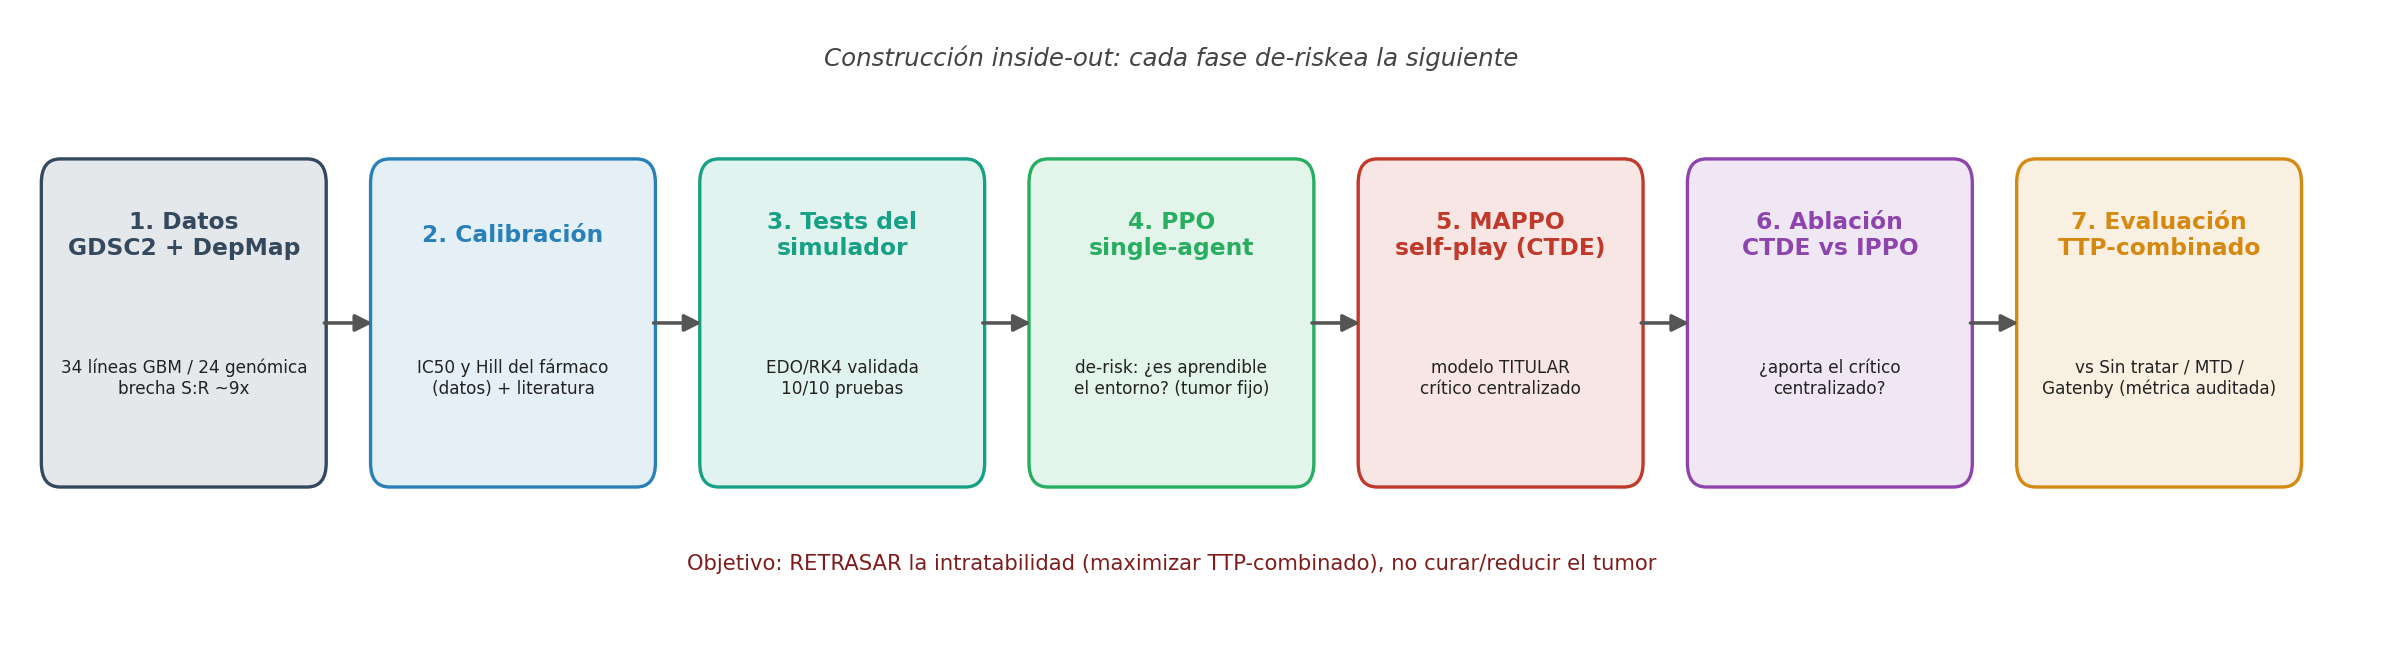
\includegraphics[width=\textwidth]{images/pipeline_diagram.png}
\caption{Pipeline experimental reproducible de GBMARL. Cada fase de-riskea la siguiente: los datos calibran el simulador, el simulador se valida con pruebas unitarias, un agente único (PPO) confirma que el entorno es aprendible antes de introducir el segundo agente, el modelo titular (MAPPO) se contrasta con su ablación (IPPO) y, finalmente, todo se evalúa con la métrica auditada frente a las líneas base. El objetivo transversal es \emph{retrasar} la intratabilidad, no reducir el tumor.}
\label{fig:pipeline}
\end{figure}

La Tabla~\ref{tab:pipeline} explicita, para cada fase, su propósito, su vínculo con el objetivo clínico (maximizar el tiempo de manejo) y qué aporta o qué riesgo elimina dentro del marco. La lógica de fondo es que un resultado multiagente solo es creíble si el sustrato sobre el que se aprende ---la dinámica, su calibración y la propia aprendibilidad del entorno--- ya fue probado por separado.

\begin{table}[H]
\centering
\caption{Fases del pipeline experimental: propósito, vínculo con el objetivo y contribución. El objetivo del marco es maximizar el TTP-combinado (retrasar la intratabilidad).}
\label{tab:pipeline}
\renewcommand{\arraystretch}{1.3}
\begin{tabular}{p{2.4cm}|p{4.0cm}|p{5.7cm}}
\textbf{Fase} & \textbf{Propósito} & \textbf{Vínculo con el objetivo y contribución} \\
\hline
1. Datos (GDSC2 + DepMap) & Recuperar líneas de glioblastoma con sensibilidad a temozolomida. & Anclan la dinámica a la biología real (brecha S:R $\approx 9\times$); sin ellos la resistencia sería un supuesto arbitrario. \\
2. Calibración & Derivar IC50 y forma de Hill de los datos; anclar el resto a literatura. & Fija la \emph{potencia} del fármaco con la que se mide cuánto se puede retrasar la progresión; separa dato de supuesto. \\
3. Tests del simulador & Probar la EDO/RK4 de forma aislada (10/10 pruebas). & Garantiza que la dinámica conserva masa y es biológicamente válida antes de aprender sobre ella. \\
4. PPO single-agent & De-riskear el entorno: ¿es aprendible contra un tumor fijo? & Verifica que la señal de recompensa induce control \emph{antes} de añadir el adversario; aísla fallos del entorno de fallos del MARL. \\
5. MAPPO self-play (CTDE) & Entrenar el modelo titular: terapia y tumor co-evolucionan. & Produce la política adaptativa que maximiza el tiempo de manejo; es la contribución central. \\
6. Ablación CTDE vs.\ IPPO & Aislar el efecto del crítico centralizado. & Atribuye causalmente la ventaja al componente CTDE, no al azar ni a otros factores. \\
7. Evaluación TTP-combinado & Comparar frente a Sin tratar, MTD y Gatenby con la métrica auditada. & Cuantifica el objetivo (días de manejo) de forma honesta y comparable; cierra el ciclo de validación. \\
\end{tabular}
\end{table}

\subsection{Por qué cada comparación}
\label{sec:porque-comparaciones}

El pipeline contiene tres comparaciones deliberadas, cada una respondiendo a una pregunta distinta. La comparación frente a las \textbf{líneas base} (Sin tratamiento, MTD y Gatenby) responde a si el aprendizaje aporta algo sobre lo ya conocido: Sin tratamiento fija el piso (la progresión natural), MTD representa el estándar clínico intuitivo de ``pegar fuerte'' y Gatenby es el competidor fuerte ---la mejor heurística adaptativa publicada---, de modo que superar a Gatenby es la prueba exigente de valor. La comparación \textbf{MAPPO frente a IPPO} (ablación) responde a si el crítico centralizado es la causa de la ventaja, manteniendo todo lo demás idéntico; sin esta comparación, atribuir el resultado a CTDE sería una conjetura. La comparación de \textbf{PPO frente al azar} (de-risk) responde a si el entorno es siquiera aprendible, y debe pasar antes de invertir esfuerzo en el aprendizaje multiagente. Reportar las tres ---y no solo la favorable--- es lo que convierte el resultado en una afirmación auditable.

\subsection{Ejecución reanudable con checkpointing intra-corrida}
\label{sec:checkpointing}

El entrenamiento adversarial a la escala de la tesis (120\,000 pasos por corrida, decenas de semillas entre el modelo titular y la ablación) excede el tiempo disponible en una sola ejecución del entorno de cómputo. Para preservar la reproducibilidad sin sacrificar la escala, el pipeline se ejecuta mediante un \textbf{arnés reanudable con checkpointing intra-corrida}: cada ventana de cómputo entrena durante un presupuesto fijo de tiempo y luego serializa un punto de control completo ---pesos de actores y críticos, estado de los optimizadores, estado de los generadores aleatorios, paso acumulado y estado del entorno---, de modo que la siguiente ventana reanuda exactamente donde la anterior se detuvo, hasta alcanzar los pasos objetivo. El rollout de entrenamiento emplea además una ruta de integración escalar de la EDO, verificada numéricamente como idéntica a la implementación vectorizada de referencia (diferencia máxima nula sobre trayectorias completas), que reduce el tiempo de cómputo sin alterar la física ni la recompensa. Este mecanismo no modifica ninguna decisión de modelado: es la maquinaria de ejecución que hace factible la corrida completa de validación reportada en la Sección~\ref{sec:res-confirmacion}.
\chapter{RESULTADOS}
\label{cap:resultados}

Este capítulo presenta los resultados experimentales de GBMARL siguiendo el orden de construcción del marco: la calibración del simulador (Sección~\ref{sec:res-calibracion}), la validación del entorno y la convergencia del aprendizaje (Sección~\ref{sec:res-aprendizaje}), la comparación frente a las líneas base con la métrica auditada (Sección~\ref{sec:res-comparacion}), el mecanismo de la política aprendida (Sección~\ref{sec:res-mecanismo}), la ablación del crítico centralizado (Sección~\ref{sec:res-ablacion}) y el análisis de sensibilidad (Sección~\ref{sec:res-sensibilidad}). La interpretación de estos hallazgos y sus implicaciones se desarrollan en el capítulo siguiente.

\section{Calibración del simulador}
\label{sec:res-calibracion}

La corrección del cruce entre GDSC2 y DepMap (normalización de claves en ambos lados) recuperó \textbf{34 líneas celulares de glioblastoma} con ensayos de sensibilidad a temozolomida, de las cuales \textbf{24} cuentan con anotación genómica completa. Esto contrasta con las 6 líneas que recuperaba la versión defectuosa del cruce por nombre, lo que confirma que aquel valor era un artefacto de mapeo y no una limitación real de los datos.

De estos ensayos se derivó una concentración inhibitoria media de la población sensible $\mathrm{IC50}_S \approx 0{,}36$ y de la población resistente $\mathrm{IC50}_R \approx 3{,}27$, es decir, una brecha de sensibilidad de aproximadamente $9\times$. El techo de muerte celular, anclado a literatura mediante la razón muerte-crecimiento, resultó en $\delta_S^{\max} = 0{,}30$ y $\delta_R^{\max} = 0{,}15$. Un hallazgo relevante de la calibración es que estos valores caracterizan a la temozolomida como un fármaco débil \emph{in vitro}, coherente con el carácter clínicamente refractario del glioblastoma. La Figura~\ref{fig:dynamics} muestra la dinámica de referencia del simulador calibrado bajo distintos regímenes de dosis.

\begin{figure}[H]
\centering
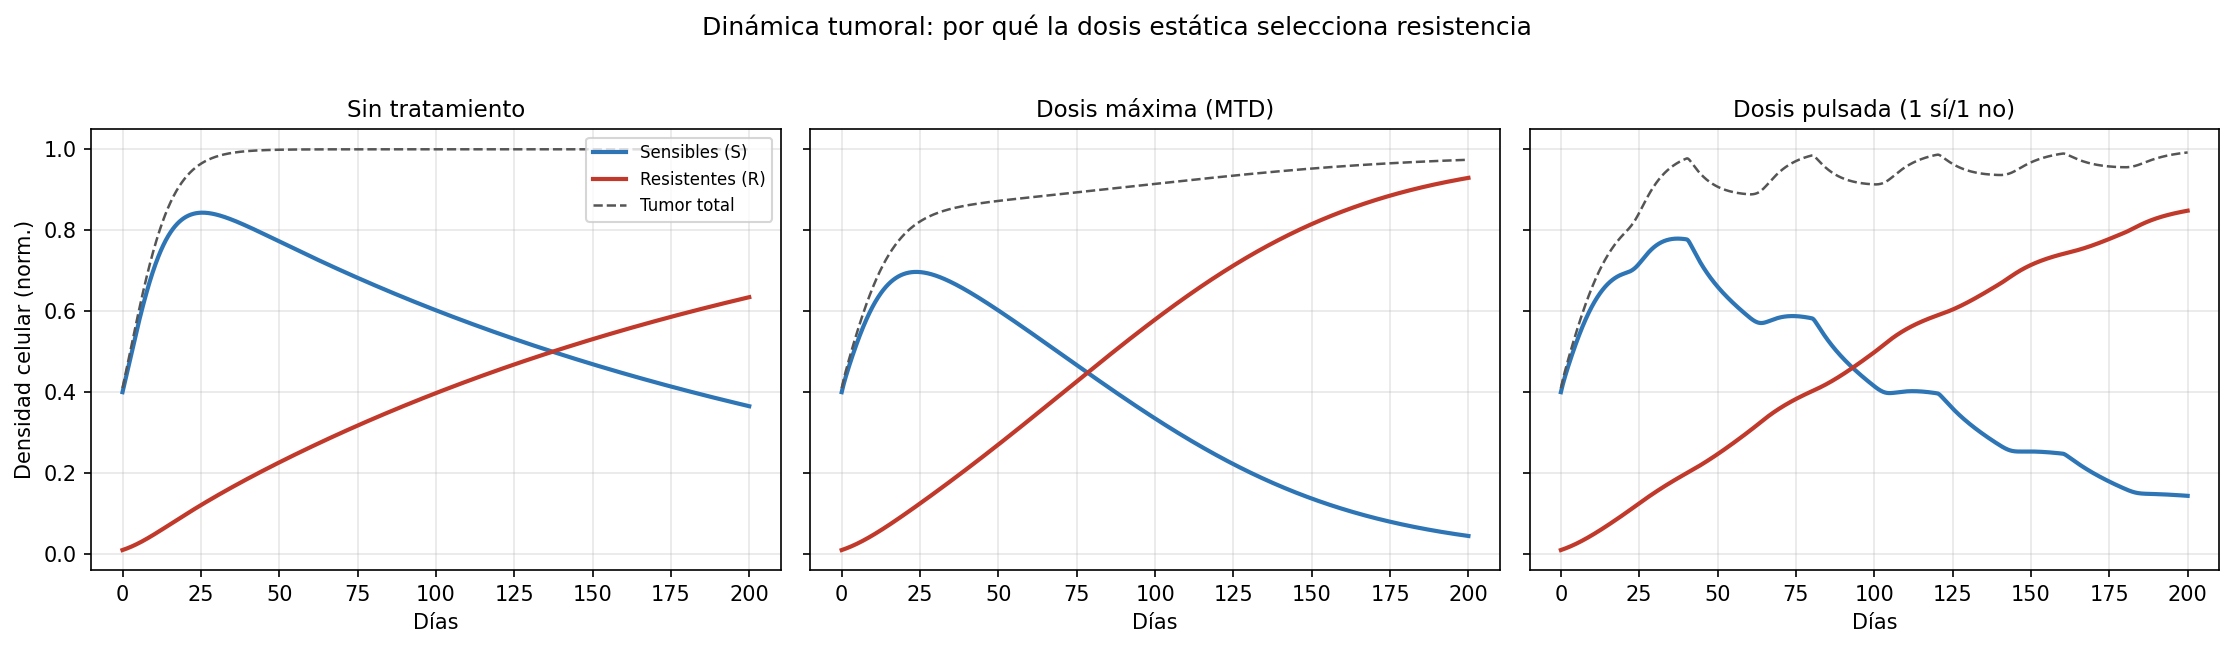
\includegraphics[width=0.85\textwidth]{images/dynamics_baseline.png}
\caption{Dinámica de referencia del simulador calibrado: evolución de las poblaciones sensible y resistente bajo distintos regímenes de dosificación.}
\label{fig:dynamics}
\end{figure}

\section{Validación del entorno y convergencia del aprendizaje}
\label{sec:res-aprendizaje}

Siguiendo la estrategia de validación incremental, se entrenó primero un agente único con PPO contra un tumor de comportamiento fijo. El retorno del agente de terapia mejoró de forma sostenida durante el entrenamiento, confirmando que el entorno es aprendible antes de introducir la complejidad multiagente.

Posteriormente, el entrenamiento adversarial por \emph{self-play} con MAPPO mostró la co-evolución de ambos agentes: el retorno de la terapia y el del tumor se incrementan conjuntamente hasta estabilizarse, como ilustra la Figura~\ref{fig:learning}. La convergencia es estable bajo el régimen determinista adoptado, lo que garantiza la reproducibilidad de cada corrida.

\begin{figure}[H]
\centering
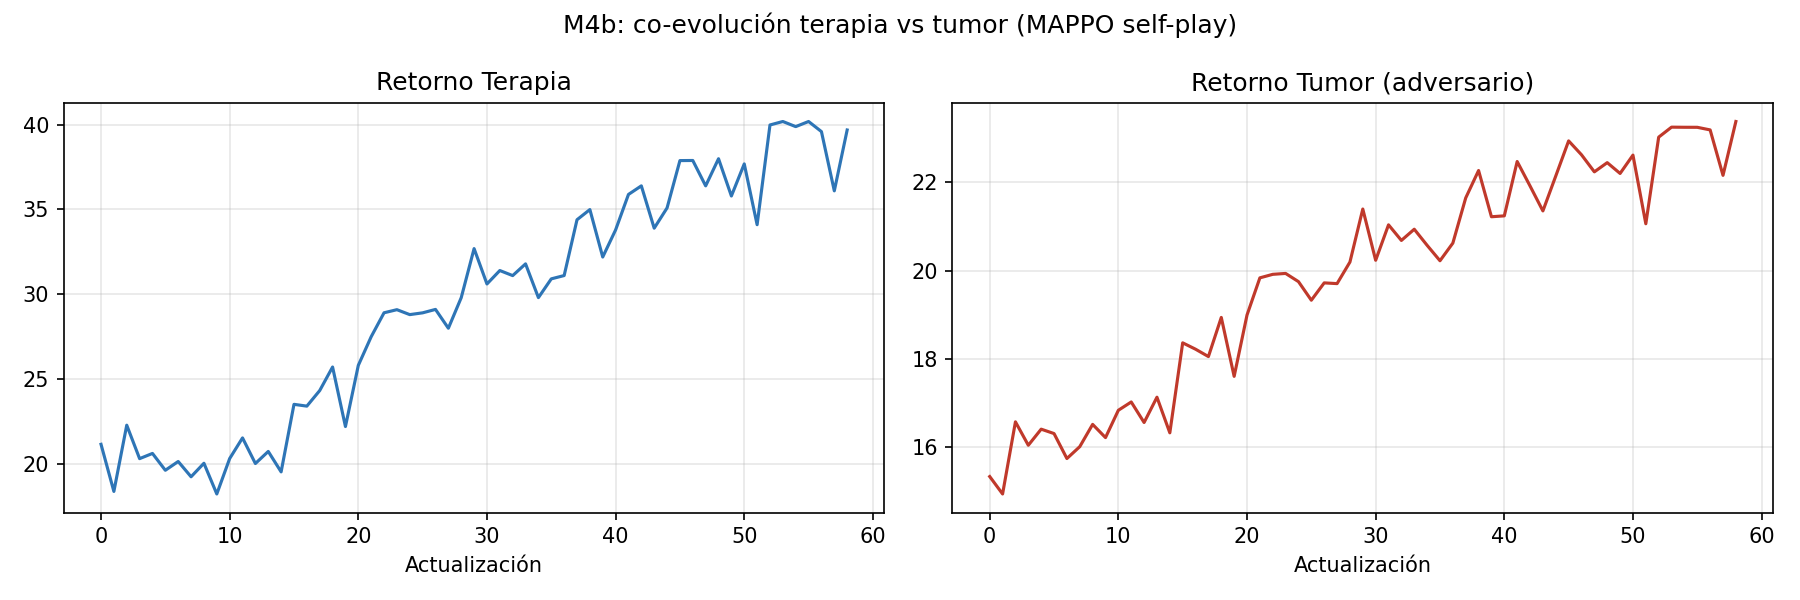
\includegraphics[width=0.95\textwidth]{images/mappo_learning_curves.png}
\caption{Curvas de aprendizaje del entrenamiento adversarial MAPPO por self-play: retorno del agente de terapia (izquierda) y del agente tumoral (derecha) a lo largo de las actualizaciones.}
\label{fig:learning}
\end{figure}

\section{Comparación frente a las líneas base}
\label{sec:res-comparacion}

La política aprendida se comparó contra tres referencias deterministas bajo la métrica de tiempo a falla combinado (TTP-combinado), reportando el modo de falla de cada estrategia. La Tabla~\ref{tab:res-baselines} resume los resultados de una evaluación representativa.

\begin{table}[H]
\centering
\caption{Comparación de estrategias bajo la métrica TTP-combinado, con el modo de falla. Métrica auditada mediante el procedimiento de diagnóstico.}
\label{tab:res-baselines}
\renewcommand{\arraystretch}{1.25}
\begin{tabular}{l|c|c|c|l}
\textbf{Estrategia} & \textbf{TTP (días)} & \textbf{Carga final} & \textbf{Frac.\ R final} & \textbf{Modo de falla} \\
\hline
Sin tratamiento     & 12  & 0.80 & 0.12 & carga progresó \\
MTD (dosis máx.)    & 13  & 0.09 & 0.52 & resistencia mayoría \\
Gatenby (adaptativa)& 27  & 0.38 & 0.53 & resistencia mayoría \\
MAPPO (aprendida)   & 41  & 0.79 & 0.51 & resistencia mayoría \\
\end{tabular}
\end{table}

Dos observaciones se desprenden de la Tabla~\ref{tab:res-baselines}. Primero, la métrica auditada revela que la ausencia de tratamiento falla por progresión de carga (día 12) mientras la fracción resistente permanece baja (0.12); todas las estrategias que tratan fallan, en cambio, por mayoría resistente. Segundo, la dosis máxima reduce la carga al mínimo (0.09) pero falla casi tan rápido como la ausencia de tratamiento (día 13), confirmando que la reducción agresiva del tumor precipita la resistencia. La política aprendida por MAPPO alcanza el mayor tiempo de manejo (41 días en esta corrida), superando a la heurística de Gatenby (27 días) y a la dosis máxima (13 días). La Figura~\ref{fig:ttp} muestra las trayectorias de carga tumoral y de fracción resistente para las cuatro estrategias.

\begin{figure}[H]
\centering
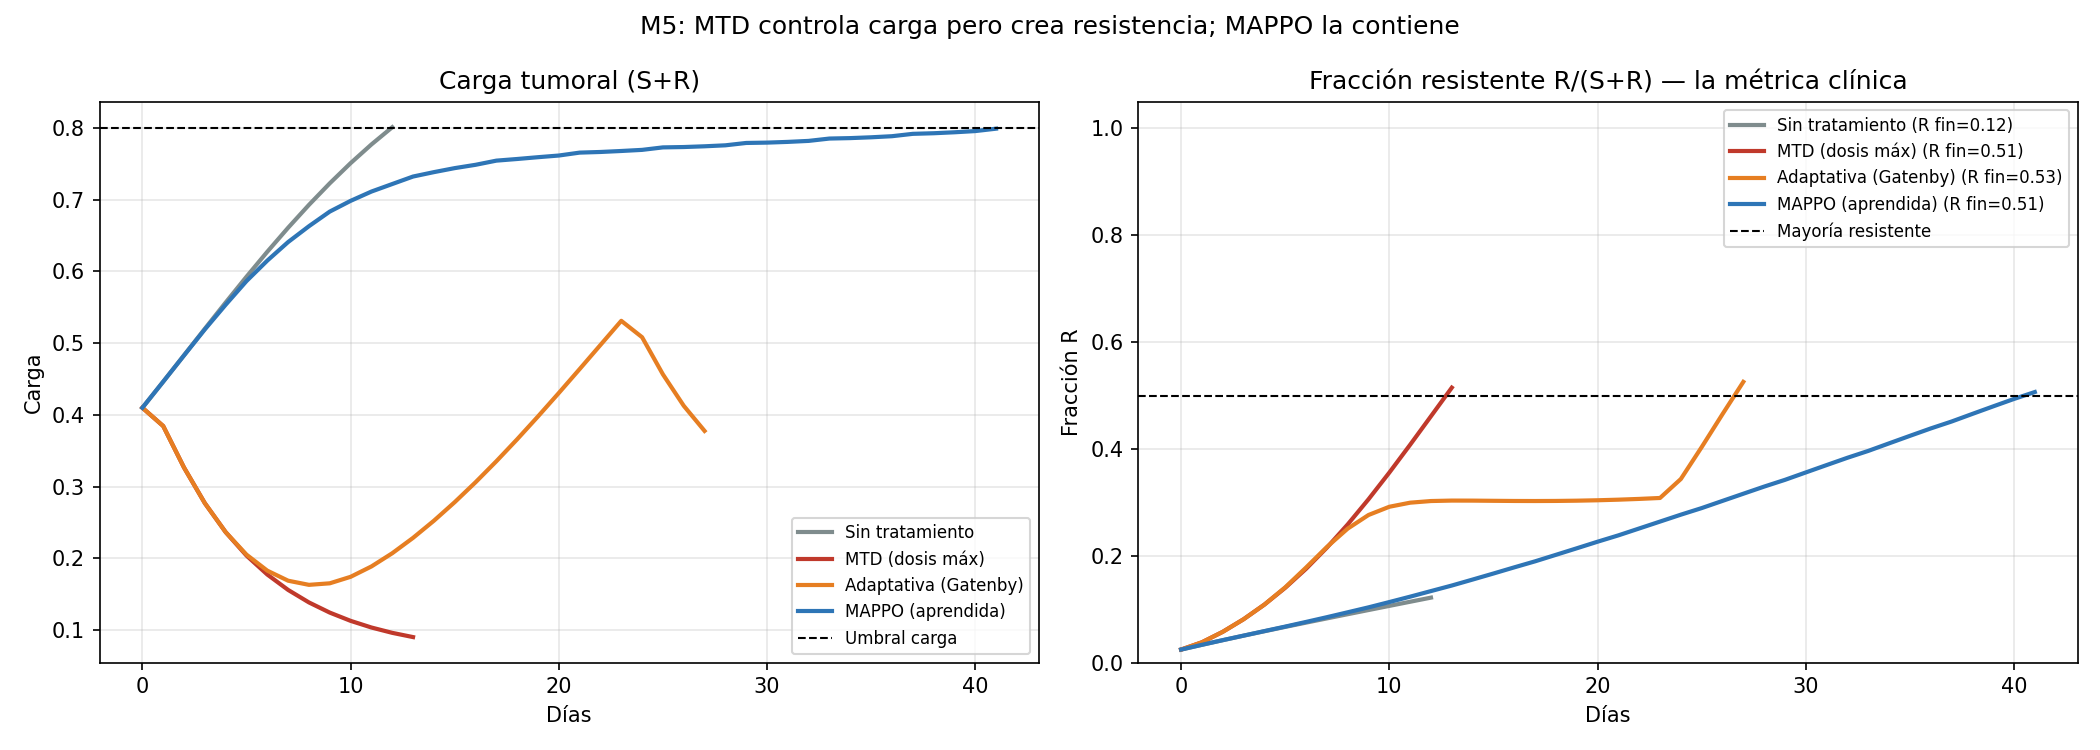
\includegraphics[width=0.95\textwidth]{images/evaluation_ttp.png}
\caption{Trayectorias de carga tumoral (izquierda) y de fracción resistente (derecha) para las cuatro estrategias. La dosis máxima controla la carga pero lleva la resistencia a su totalidad; la política aprendida retrasa la dominancia resistente.}
\label{fig:ttp}
\end{figure}

\subsection{Validación multi-semilla y bimodalidad}

Dado que el entrenamiento adversarial por \emph{self-play} es estocástico, el resultado se validó sobre 15 semillas independientes. La distribución de los tiempos de manejo es \textbf{bimodal}: una fracción de las corridas converge a una cuenca con tiempos en el rango de 25 a 33 días, mientras que otra fracción alcanza una cuenca superior, en torno a los 41 días. Reportamos por tanto ambos valores con igual peso: la \textbf{mejor corrida alcanza 41 días}, y la \textbf{media sobre las 15 semillas es de $33{,}5 \pm 5{,}8$ días} (mediana 32). La bimodalidad refleja que la co-evolución se asienta en distintos equilibrios según la inicialización, un fenómeno conocido del aprendizaje multiagente por self-play.

En ambas lecturas, la política aprendida supera a las dos líneas base de forma estadísticamente significativa (Tabla~\ref{tab:res-multisemilla}): frente a Gatenby ($p < 0{,}001$) y frente a la dosis máxima ($p < 0{,}001$). La Figura~\ref{fig:validation} muestra la comparación con barras de error.

\begin{table}[H]
\centering
\caption{Validación multi-semilla ($n=15$) del TTP-combinado. Las líneas base son deterministas. Significancia de la política aprendida frente a cada línea base.}
\label{tab:res-multisemilla}
\renewcommand{\arraystretch}{1.25}
\begin{tabular}{l|c|c}
\textbf{Estrategia} & \textbf{TTP (días)} & \textbf{Significancia} \\
\hline
MTD (dosis máx.)     & 13                       & --- \\
Gatenby (adaptativa) & 27                       & --- \\
MAPPO (mejor corrida)& 41                       & --- \\
MAPPO (media, $n=15$)& $33{,}5 \pm 5{,}8$ (mediana 32) & $p<0{,}001$ vs.\ MTD y Gatenby \\
\end{tabular}
\end{table}

\begin{figure}[H]
\centering
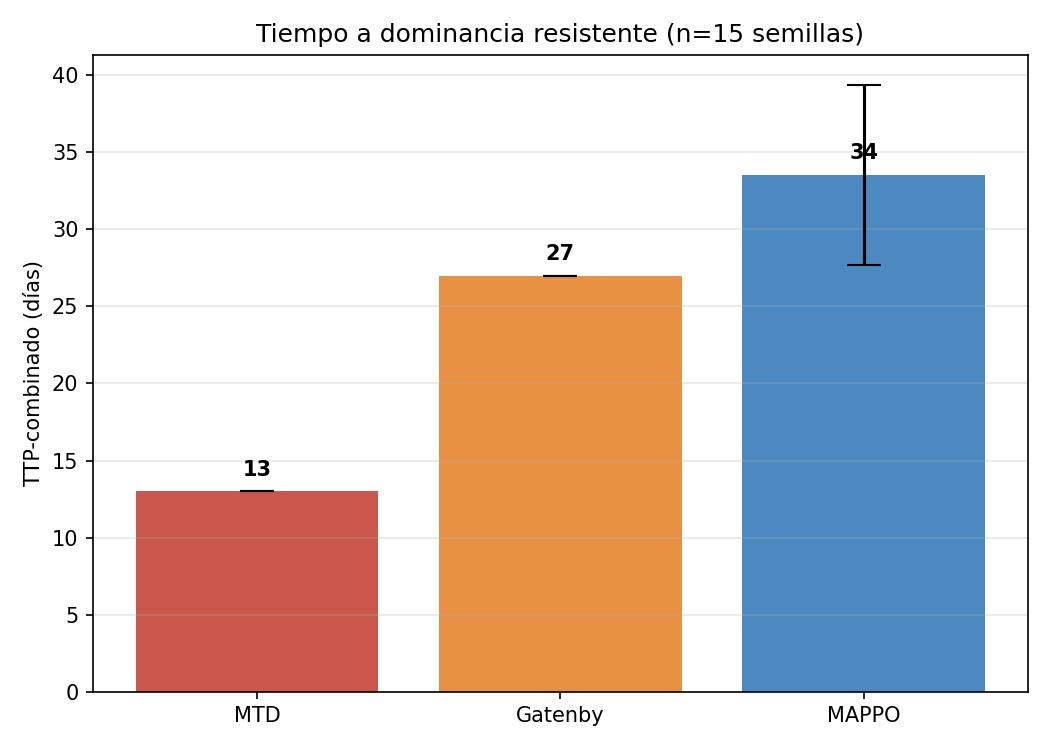
\includegraphics[width=0.6\textwidth]{images/validation_seeds.png}
\caption{Validación multi-semilla del TTP-combinado ($n=15$). La política aprendida supera a ambas líneas base deterministas; la barra de error refleja la dispersión bimodal del self-play.}
\label{fig:validation}
\end{figure}

\section{Mecanismo de la política aprendida}
\label{sec:res-mecanismo}

La inspección de las políticas de la cuenca superior revela el mecanismo descubierto por el agente. La Figura~\ref{fig:mecanismo} muestra que la política aplica una \textbf{dosificación pulsada e intermitente}: tras un periodo inicial, la dosis oscila entre valores bajos y nulos en lugar de mantenerse al máximo. Como consecuencia, la población sensible se mantiene en una densidad elevada que compite con la resistente y frena su expansión, mientras la fracción resistente crece lentamente hasta cruzar el umbral de mayoría. Este patrón corresponde al principio de la terapia adaptativa ---preservar una población sensible competidora--- redescubierto de forma autónoma por el agente, sin haber sido programado explícitamente.

\begin{figure}[H]
\centering
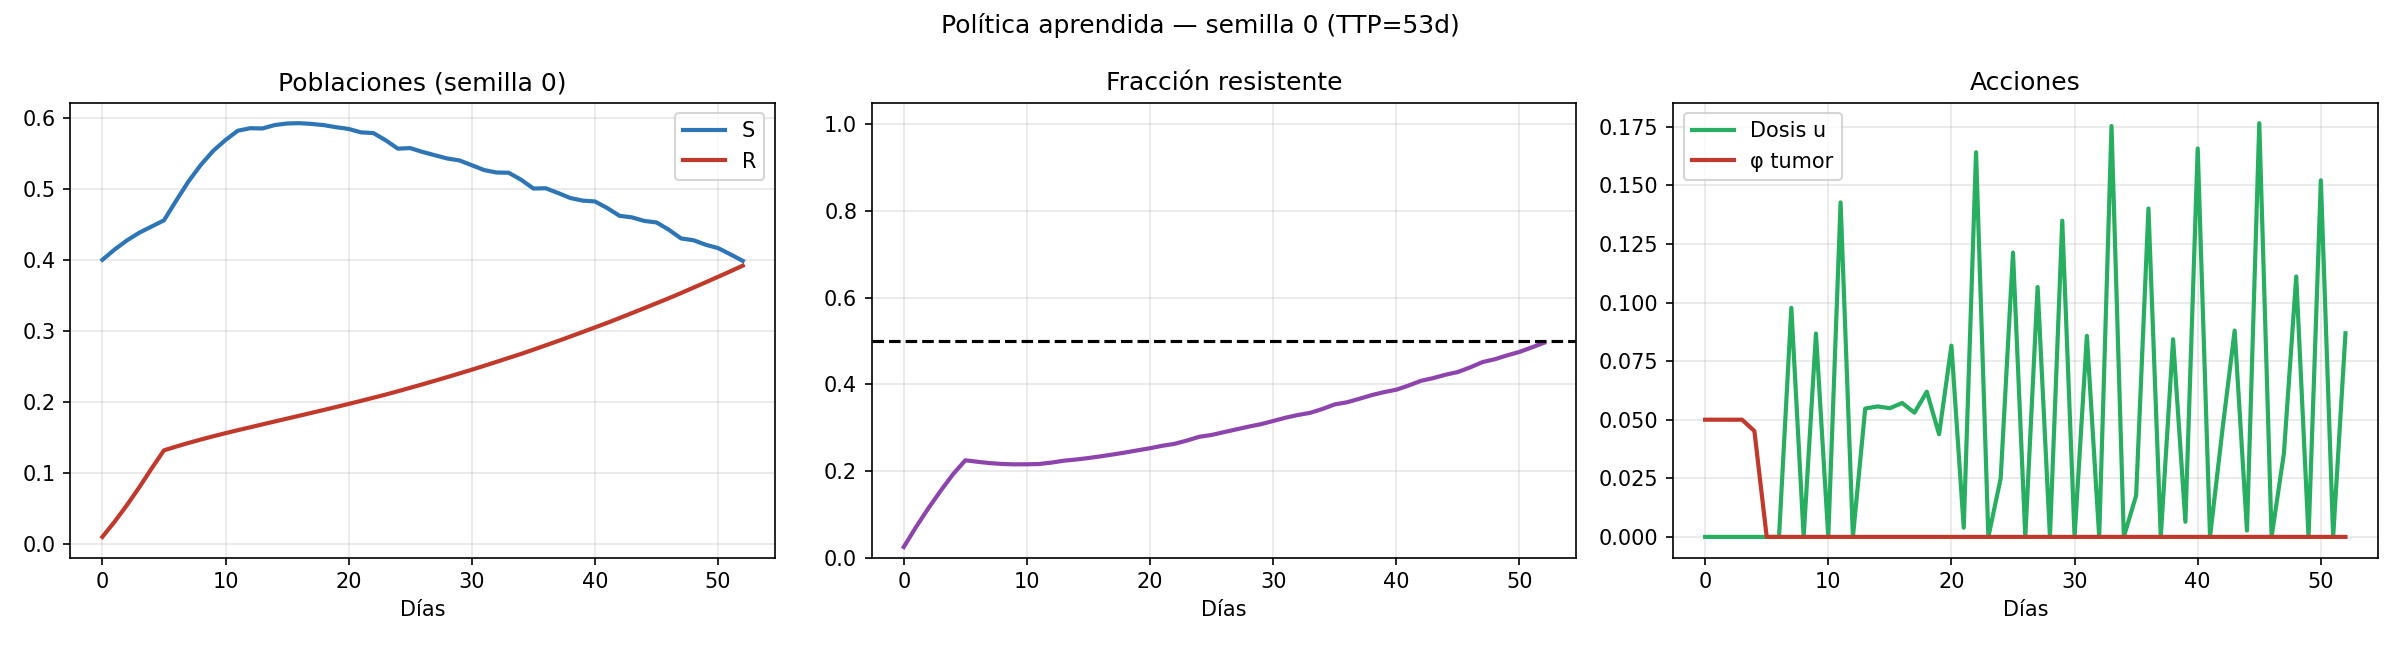
\includegraphics[width=0.95\textwidth]{images/policy_seed0.png}
\caption{Política aprendida de la cuenca superior: poblaciones (izquierda), fracción resistente (centro) y acciones de dosis y transición (derecha). La dosificación pulsada preserva la población sensible competidora.}
\label{fig:mecanismo}
\end{figure}

\section{Ablación del crítico centralizado (CTDE vs.\ IPPO)}
\label{sec:res-ablacion}

Para aislar la contribución del crítico centralizado, se comparó MAPPO (crítico condicionado al estado conjunto) con IPPO (crítico con observación local), manteniendo idénticos el actor, la observación de ejecución y todos los hiperparámetros. La verificación de la arquitectura confirmó que el cambio de variante modifica efectivamente la dimensión de entrada del crítico (3 para MAPPO, 2 para IPPO).

Bajo la métrica auditada, MAPPO alcanza un tiempo de manejo medio de $34{,}8 \pm 5{,}7$ días frente a $30{,}2 \pm 2{,}9$ días de IPPO (Tabla~\ref{tab:res-ablacion}). La diferencia favorece al crítico centralizado, aunque su margen es estrecho. Un contraste cualitativo es informativo: las corridas de IPPO tienden a fallar por progresión de carga, mientras que las mejores corridas de MAPPO fallan por mayoría resistente, lo que indica que MAPPO sostiene el control de la carga durante más tiempo antes de ceder a la resistencia.

\begin{table}[H]
\centering
\caption{Ablación del crítico centralizado. Ambas variantes comparten actor, observación de ejecución e hiperparámetros; solo difiere la entrada del crítico.}
\label{tab:res-ablacion}
\renewcommand{\arraystretch}{1.25}
\begin{tabular}{l|c|l}
\textbf{Variante} & \textbf{TTP (días)} & \textbf{Modo de falla predominante} \\
\hline
MAPPO (crítico centralizado, CTDE) & $34{,}8 \pm 5{,}7$ & resistencia mayoría \\
IPPO (crítico local)               & $30{,}2 \pm 2{,}9$ & carga progresó \\
\end{tabular}
\end{table}

\begin{figure}[H]
\centering
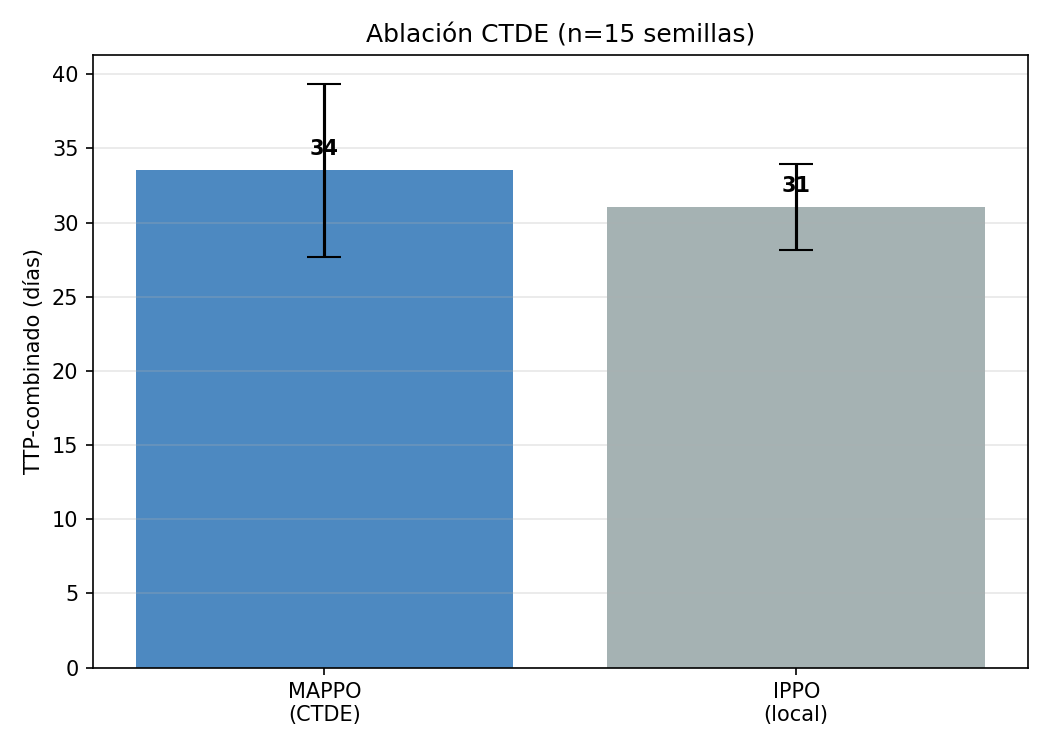
\includegraphics[width=0.6\textwidth]{images/ablation_ctde.png}
\caption{Ablación CTDE: MAPPO (crítico centralizado) frente a IPPO (crítico local) bajo el TTP-combinado.}
\label{fig:ablacion}
\end{figure}

\section{Análisis de sensibilidad}
\label{sec:res-sensibilidad}

Se varió, una a la vez, cada una de las seis constantes elegidas a mano alrededor de su valor por defecto, recalculando el TTP-combinado de las tres estrategias en cada punto. La Tabla~\ref{tab:res-sensibilidad} resume el rango de la política aprendida frente a las líneas base. En las seis constantes y en todo el rango evaluado, la política aprendida se mantiene por encima de la heurística de Gatenby y de la dosis máxima; el ordenamiento $\text{MAPPO} > \text{Gatenby} > \text{MTD}$ no se invierte en ningún punto.

\begin{table}[H]
\centering
\caption{Análisis de sensibilidad. Rango del TTP-combinado de MAPPO al variar cada constante $\pm 30\%$ (o entre valores razonables), frente al rango de las líneas base.}
\label{tab:res-sensibilidad}
\renewcommand{\arraystretch}{1.25}
\begin{tabular}{l|c|c|c}
\textbf{Constante variada} & \textbf{MAPPO (rango)} & \textbf{Gatenby} & \textbf{MTD} \\
\hline
$\phi_{\max}$ (fuerza adversario)    & 30.0--39.3 & 27        & 13 \\
$\theta_{\text{prog}}$ (umbral carga)& 32.3--44.0 & 27        & 13 \\
$\rho_{\text{may}}$ (umbral mayoría) & 28.3--40.3 & 25--29    & 11--15 \\
$w_{\text{tox}}$ (toxicidad)         & 37.7       & 27        & 13 \\
$\delta_S^{\max}$ (potencia fármaco) & 33.7--38.3 & 27--29    & 10--19 \\
$\mathrm{IC50}_R$ (brecha resistencia)& 36.0--39.7 & 27--28   & 13--15 \\
\end{tabular}
\end{table}

El parámetro más sensible es la potencia del fármaco $\delta_S^{\max}$: al aumentarla, la dosis máxima falla más rápido (de 19 a 10 días) por selección acelerada de resistencia, mientras que la política aprendida y la heurística de Gatenby se mantienen estables. La Figura~\ref{fig:sensibilidad} presenta los seis barridos.

\begin{figure}[H]
\centering
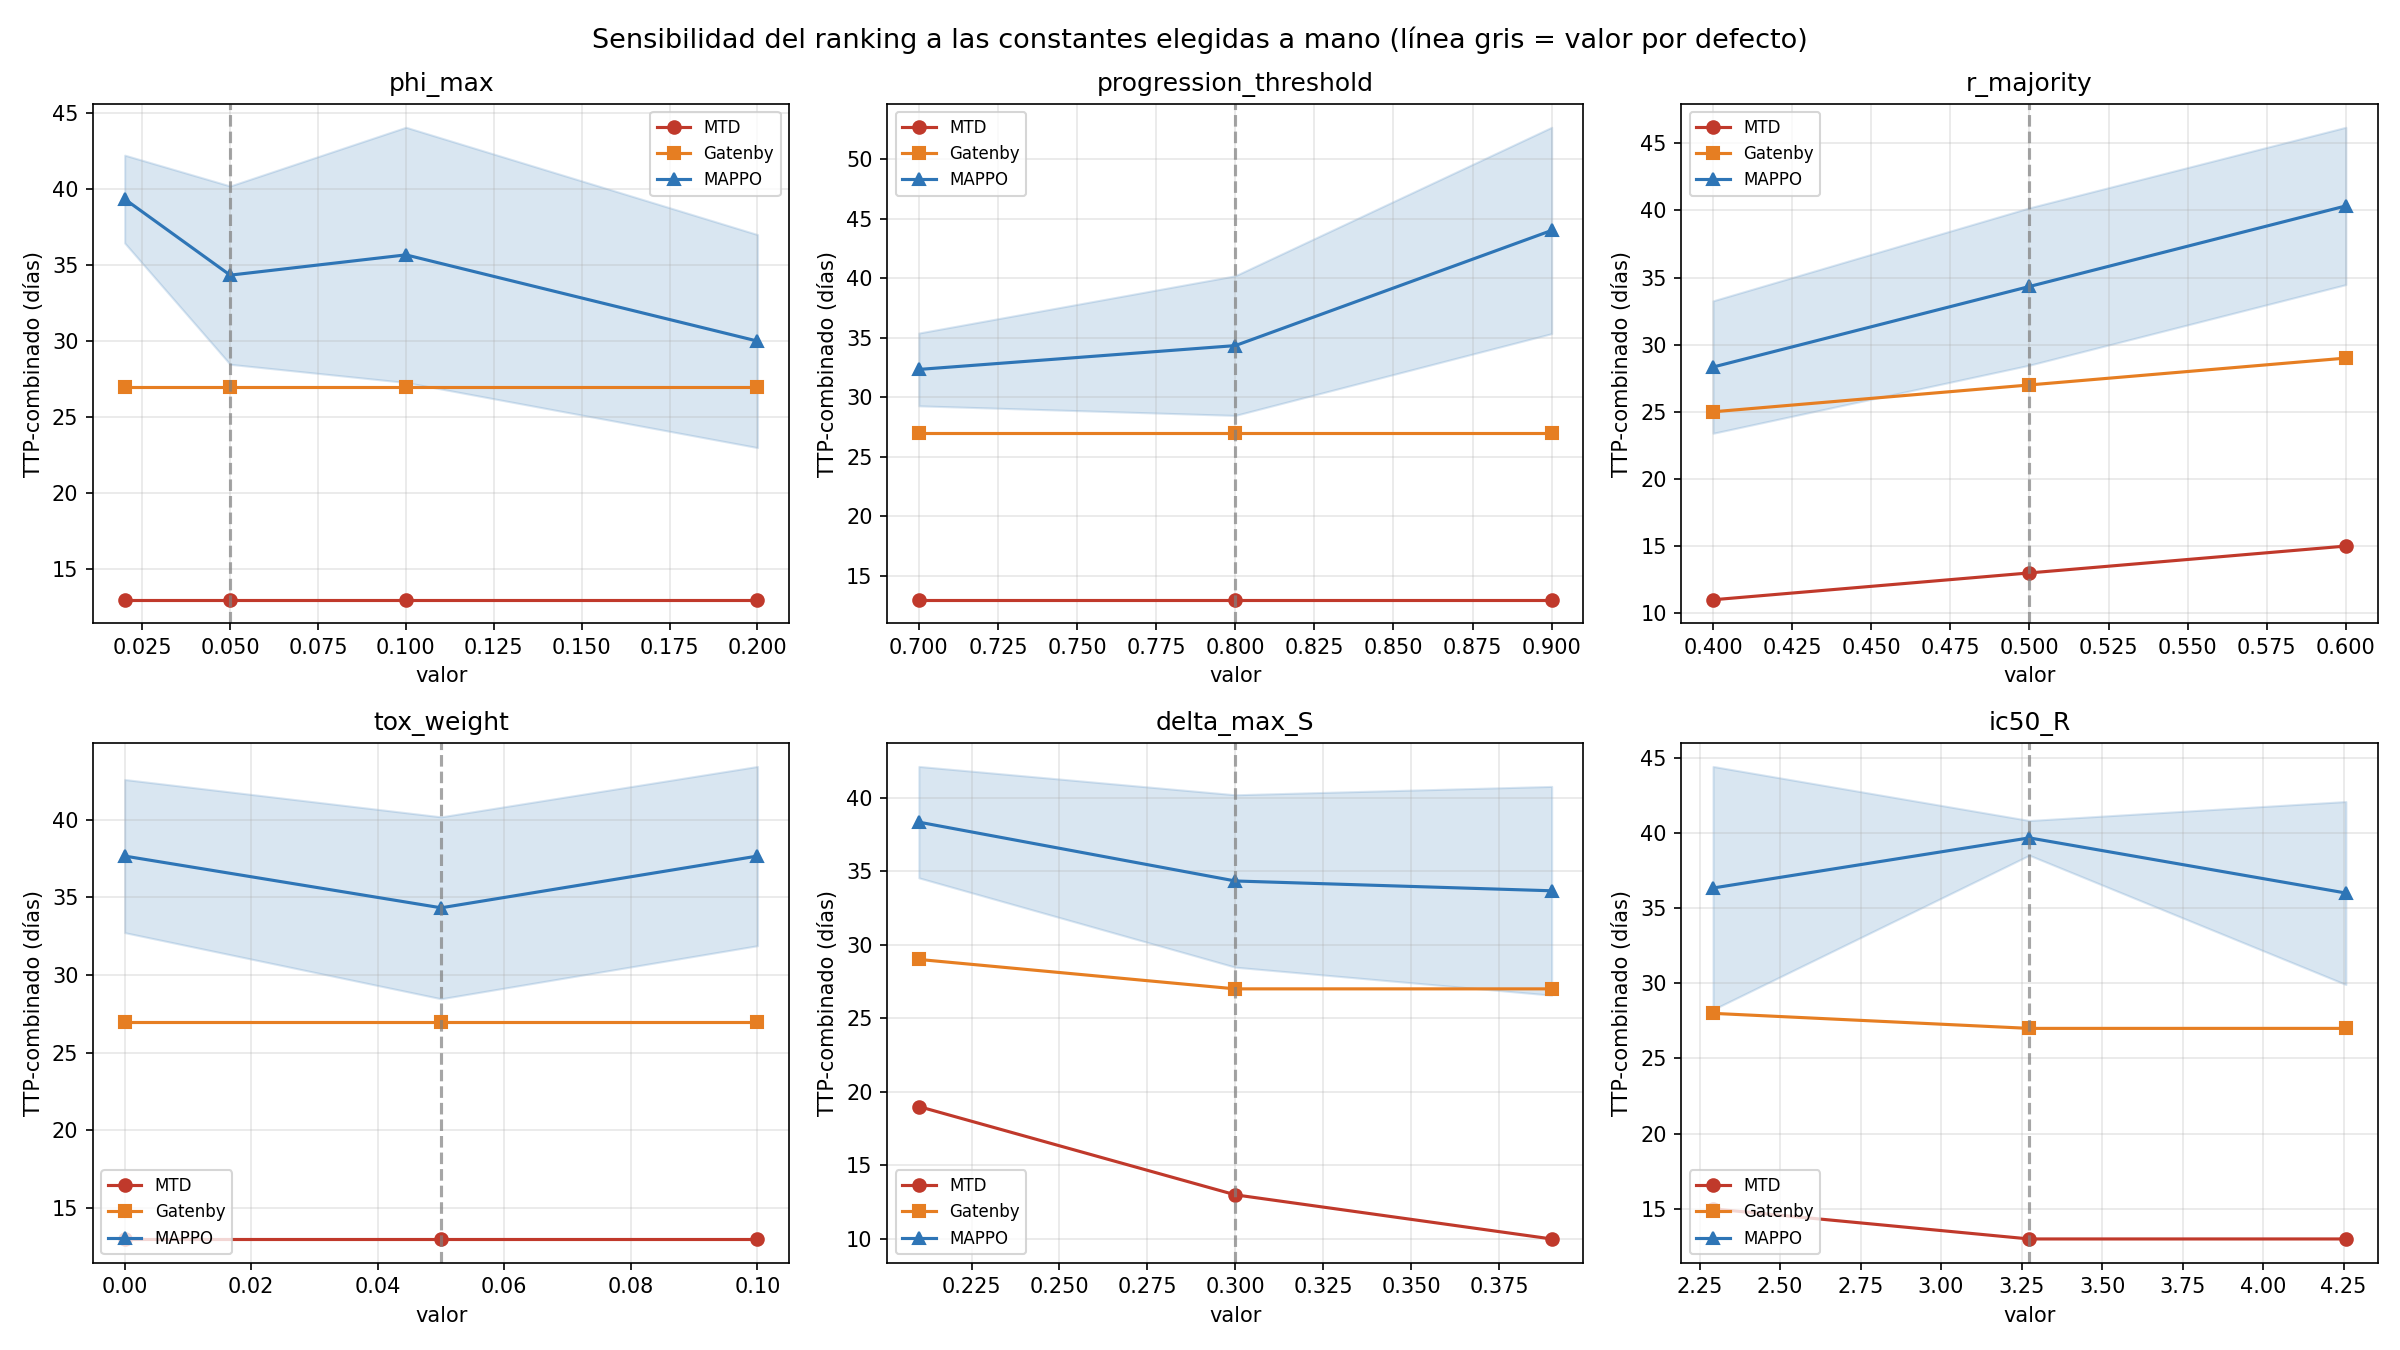
\includegraphics[width=0.95\textwidth]{images/sensitivity.png}
\caption{Análisis de sensibilidad sobre las seis constantes elegidas a mano. La curva de la política aprendida (azul) se mantiene por encima de Gatenby y de la dosis máxima en todo el rango; la línea vertical gris marca el valor por defecto.}
\label{fig:sensibilidad}
\end{figure}

\section{Confirmación con la corrida completa reproducible}
\label{sec:res-confirmacion}

Para verificar que los hallazgos no dependen de la maquinaria de cómputo, se reejecutó el pipeline completo de extremo a extremo bajo el arnés reanudable con checkpointing intra-corrida descrito en la Sección~\ref{sec:checkpointing}: el modelo titular y las dos ramas de la ablación se entrenaron a la escala plena de \textbf{120\,000 pasos}, con \textbf{cinco semillas independientes} por variante, y se evaluaron con la métrica TTP-combinado auditada. Las líneas base, al ser deterministas, reprodujeron sus valores de forma exacta (Sin tratamiento 12 días, MTD 13 días, Gatenby 27 días), lo que confirma la integridad de la reejecución.

La Tabla~\ref{tab:res-confirmacion} reporta el tiempo de manejo por semilla. La lectura honesta para una distribución bimodal es la \textbf{tasa de éxito} y la \textbf{mediana}, no el promedio. MAPPO-CTDE supera a la heurística de Gatenby en las \textbf{cinco de cinco} semillas (mediana 33 días, mejor corrida 41), mientras que IPPO lo hace en \textbf{cuatro de cinco} (mediana 30 días). El ordenamiento $\text{MAPPO} > \text{IPPO} > \text{Gatenby} > \text{MTD} > \text{Sin tratar}$ se mantiene, reproduciendo el hallazgo central de la validación multi-semilla ($n=15$) con una corrida totalmente reproducible.

\begin{table}[H]
\centering
\caption{Corrida completa reproducible (120\,000 pasos, $n=5$ semillas por variante). TTP-combinado por semilla y tasa de éxito frente a Gatenby (27 días). Para la distribución bimodal se reporta mediana y tasa de éxito, no media$\pm$desv.}
\label{tab:res-confirmacion}
\renewcommand{\arraystretch}{1.25}
\begin{tabular}{l|c|c|c|c|c|c|c}
\textbf{Variante} & \textbf{s0} & \textbf{s1} & \textbf{s2} & \textbf{s3} & \textbf{s4} & \textbf{Mediana} & \textbf{Éxito $>$Gatenby} \\
\hline
MAPPO (CTDE) & 41 & 32 & 31 & 33 & 41 & \textbf{33} & \textbf{5/5} \\
IPPO (local) & 31 & 29 & 25 & 30 & 40 & 30 & 4/5 \\
\end{tabular}
\end{table}

La Figura~\ref{fig:confirmacion} contrasta las medianas de ambas variantes de RL frente a las tres líneas base (panel a) y muestra la dispersión por semilla que evidencia la bimodalidad (panel b): ambas variantes presentan una mayoría de corridas agrupadas en torno a los 30--33 días y semillas aisladas que alcanzan la cuenca superior de 40--41 días, justificando el reporte por tasa de éxito en lugar de promedios. Coherente con el mecanismo descrito en la Sección~\ref{sec:res-mecanismo}, la dosis media aprendida en todas las semillas exitosas es baja (en torno a 0.05--0.06), confirmando la dosificación pulsada como patrón estable del aprendizaje.

\begin{figure}[H]
\centering
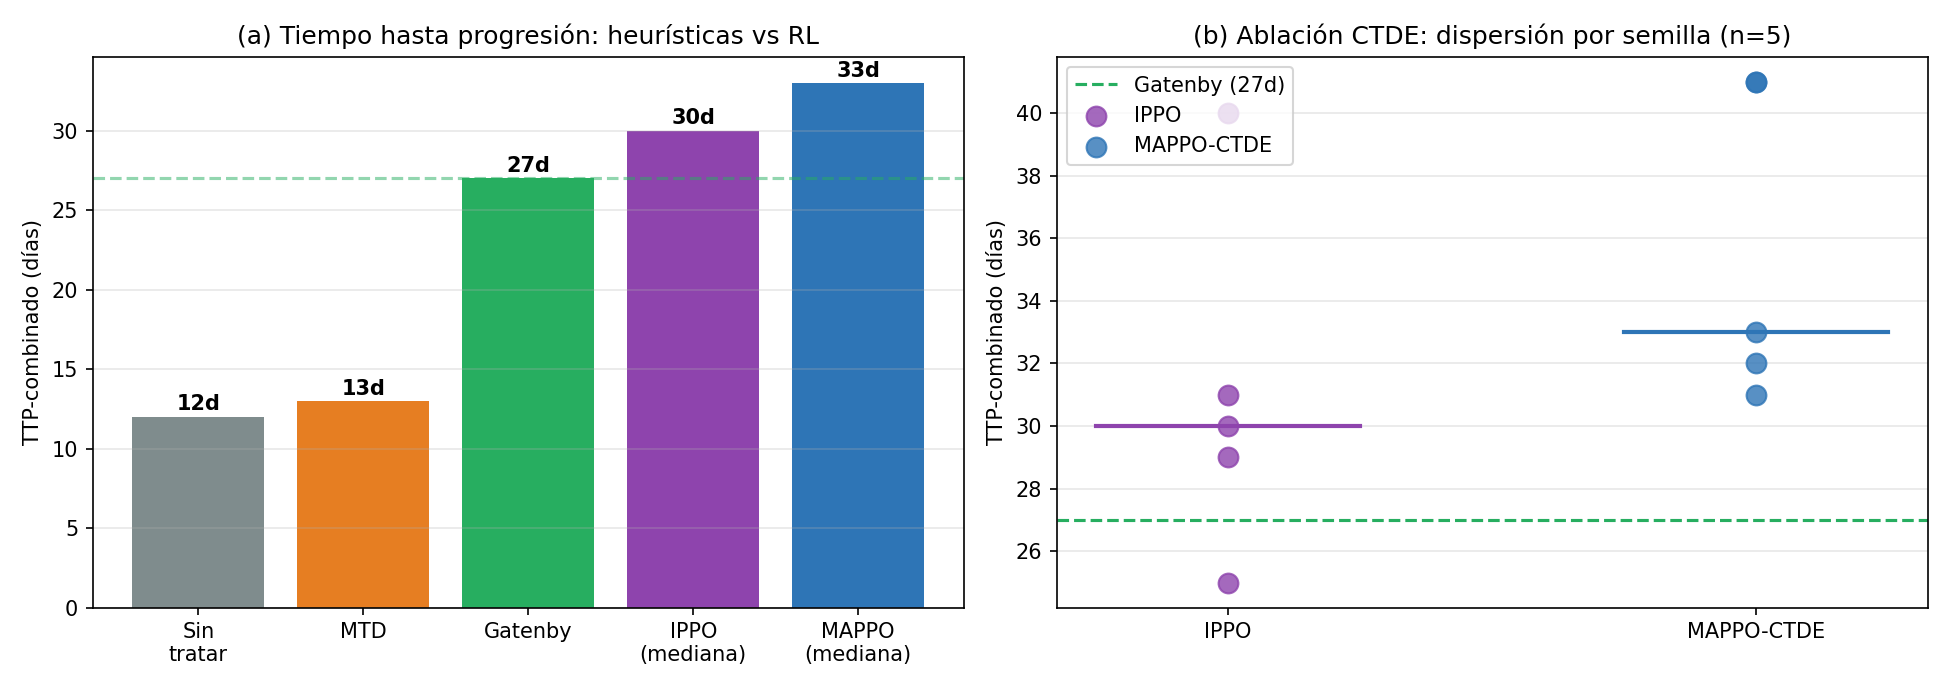
\includegraphics[width=\textwidth]{images/resultados_full_120k.png}
\caption{Corrida completa reproducible (120\,000 pasos). (a) Mediana del TTP-combinado de las variantes de RL frente a las líneas base; la línea discontinua marca a Gatenby. (b) Dispersión por semilla ($n=5$): la mayoría de corridas se agrupa cerca de la mediana y semillas aisladas alcanzan la cuenca superior (bimodalidad), por lo que el resultado se reporta como tasa de éxito.}
\label{fig:confirmacion}
\end{figure}

En conjunto, los resultados muestran que la política aprendida por GBMARL extiende el tiempo de manejo clínico de forma significativa frente a las dos líneas base, mediante un mecanismo de dosificación pulsada interpretable, con una ventaja modesta del crítico centralizado y un ordenamiento robusto frente a la variación de los hiperparámetros, y ese ordenamiento se reproduce en una corrida completa de extremo a extremo bajo control de reproducibilidad.
\input{secciones/conclusiones}
\input{secciones/recomendaciones} % sección opcional

%% ============================================================================
\renewcommand{\bibname}{\hfill\Large\bf{REFERENCIAS BIBLIOGRÁFICAS}\hfill}

\bibliographystyle{IEEEtran} % Estableciendo el estilo de citas IEEEtram.

\bibliography{referencias} % Recibe las referencias de IEEE

\input{secciones/anexos}

\end{document}
